% ----------------------------------------------------
\begin{frame}
  \titlepage
\end{frame}
% ----------------------------------------------------
\note{Presentarse. Mencionar la web del curso y los horarios de cada grupo.}

% ----------------------------------------------------
\begin{frame}[plain]
  \begin{tikzpicture}[remember picture, overlay]
    \node[at = (current page.center), yshift = 0cm] (cover) {%
      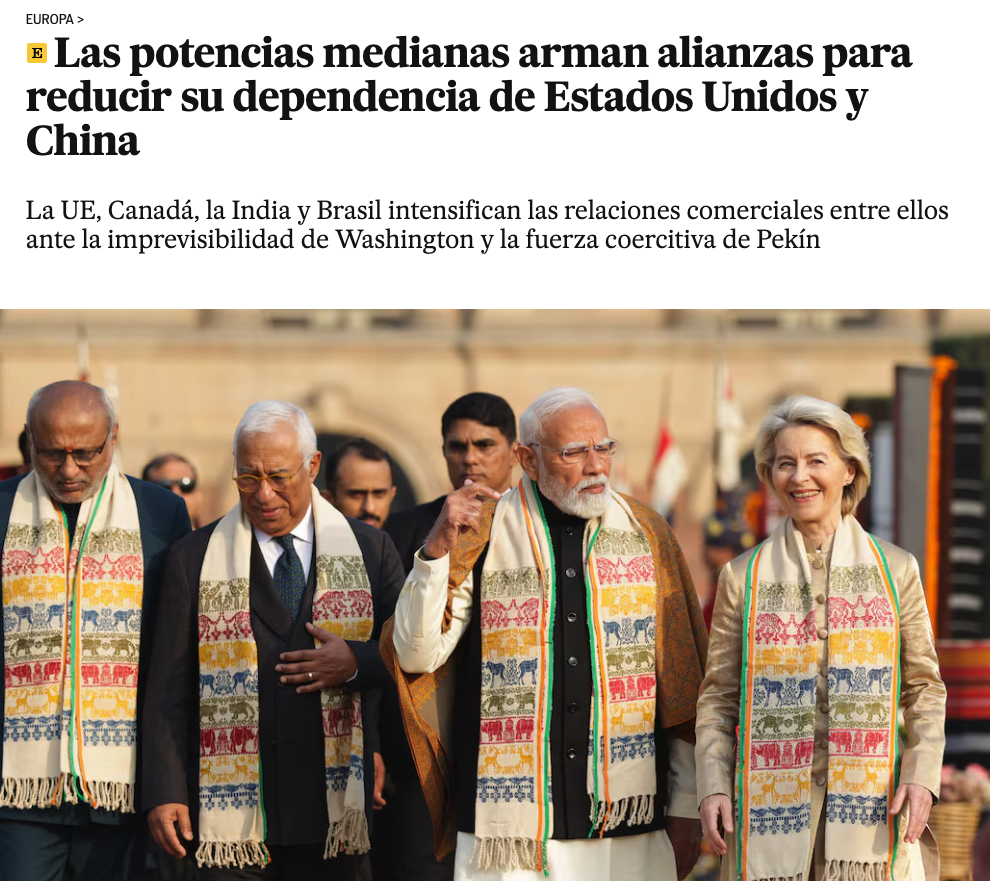
\includegraphics[keepaspectratio, height=\paperheight]{../img/potencias_medianas}};
  \end{tikzpicture}
\end{frame}
% ----------------------------------------------------
\note{Mapa de potencias medianas. Preguntar a los estudiantes qué ven y qué les llama la atención.}

% ----------------------------------------------------
\begin{frame}
\frametitle{Qué está pasando y qué ha cambiado?}
\centering

\begin{itemize}
  \item Qué está pasando?
  \item<2-> Qué le llamaría la atención del mundo de hoy a alguien que lo mirase desde hace \textbf{25 años}?
  \item<3-> Y a alguien de hace \textbf{50 años}?
\end{itemize}

\end{frame}
% ----------------------------------------------------
\note{Discusión abierta. Dejar que los estudiantes hablen. Guiar hacia: ascenso de China, guerra en Ucrania, crisis del multilateralismo, cambio climático, redes sociales y desinformación.}

% ----------------------------------------------------
\begin{frame}
\frametitle{El largo plazo}
\centering

\begin{itemize}
  \item Qué diría del mundo de hoy alguien que viviese sobre el año \textbf{1500}?
\end{itemize}

\end{frame}
% ----------------------------------------------------
\note{Transición hacia la parte histórica. Alguien de 1500 no reconocería el sistema de Estados, la economía global, la tecnología. Usar como puente hacia la cronología.}

% ====================================================
\section{Syllabus}
% ====================================================

% ----------------------------------------------------
\begin{frame}
\frametitle{Estructura del curso}
\centering

\footnotesize
\begin{tabular}{lll}
\textit{\scriptsize Bloque} & \textit{\scriptsize Fecha} & \textit{\scriptsize Tema} \\
\hline
\textit{Introducción} & 3 feb & El mundo hoy \\
  & 10 feb & Actores e intereses \\
\hline
\textit{Guerra y violencia} & 17 feb & El problema de la guerra \\
  & 24 feb & Guerras y organizaciones \\
  & 3 mar & Terrorismo \\
\hline
\textit{Normas} & 10 mar & Leyes, normas y DDHH \\
\hline
\multicolumn{3}{c}{\textbf{Examen parcial: 17 de marzo}} \\
\hline
\textit{Economía política int.} & 24 mar & Comercio internacional \\
  & 7 abr & Finanzas y dinero \\
  & 14 abr & Desarrollo económico \\
\hline
\textit{General} & 21 abr & Futuro y problemas emergentes \\
  & 28 abr & \textit{Clase de reserva} \\
  & 5 may & \textit{Presentaciones} \\
\end{tabular}

\end{frame}
% ----------------------------------------------------
\note{Repasar el programa brevemente. Mencionar el examen parcial (17 marzo) y que es opcional (elimina materia). Semana Santa: semana del 31 de marzo.}

% ----------------------------------------------------
\begin{frame}
\frametitle{Recursos}
\centering

\begin{itemize}
  \item \textbf{Web:} \url{https://franvillamil.github.io/pol_mundial/}
  \item \textbf{Libro de texto:} Frieden, Lake y Schultz, \textit{World Politics: Interests, Interactions, Institutions} (4a ed., 2019)
  \item \textbf{Lecturas complementarias:} se irán publicando en la web del curso y en Aula Global
\end{itemize}

\end{frame}
% ----------------------------------------------------
\note{El libro no es obligatorio pero sí muy recomendable. Las lecturas complementarias se van subiendo a la web y a Aula Global.}

% ----------------------------------------------------
\begin{frame}
\frametitle{Evaluación}
\centering

\begin{itemize}
  \item \textbf{20\%} -- Actividades seminarios
  \item \textbf{30\%} -- Presentación en grupo
  \item \textbf{50\%} -- Examen final
\end{itemize}

\end{frame}
% ----------------------------------------------------
\note{Tres componentes. Enfatizar que el examen pesa la mitad de la nota.}

% ----------------------------------------------------
\begin{frame}
\frametitle{Actividades seminarios (20\%)}
\centering

\begin{itemize}
  \item Varias actividades con entrega durante los seminarios
  \item Mide asistencia y compromiso activo
\end{itemize}

\end{frame}
% ----------------------------------------------------
\note{Seminarios con Luis Azores. Actividades variadas con entrega. Asistencia importa.}

% ----------------------------------------------------
\begin{frame}
\frametitle{Presentación en grupo (30\%)}
\centering

\begin{itemize}
  \item Grupos de 3--4 personas
  \item Tema relacionado con el temario (a confirmar con el profesor)
  \item 2--3 sesiones al final del curso
\end{itemize}

\vspace{15pt}

\begin{center}
\begin{tabular}{|c|c|c|}
\hline
& \textbf{Grupo 88} & \textbf{Grupo 188} \\
\hline
1er día: & Jueves 23/04 & Viernes 24/04 \\
2do día: & Jueves 30/05 & \textit{Martes 05/05} \\
3er día: & \textit{Martes 08/05} & \textit{Martes 08/05} \\
\hline
\end{tabular}
\end{center}

\end{frame}
% ----------------------------------------------------
\note{Grupos de 3--4 personas. Confirmar tema con el profesor. Las fechas en cursiva son en horario de magistral (clase de reserva).}

% ----------------------------------------------------
\begin{frame}
\frametitle{Examen final (50\%) y examen parcial}
\centering

\begin{itemize}
  \item Dos preguntas a desarrollar, escritas a mano (1 hora)
  \item Se pueden usar apuntes y libros en papel
  \item \textbf{No} dispositivos electrónicos
  \item Examen parcial opcional a mitad del cuatrimestre (elimina materia)
\end{itemize}

\end{frame}
% ----------------------------------------------------
\note{Examen open-book (papel). Sin electrónicos. El parcial es opcional: si lo haces bien, eliminas materia de la primera pregunta del final. La decisión de eliminar se toma ANTES del final.}


% ====================================================
\section{El mundo hasta la Revolución Francesa}
% ====================================================

% ----------------------------------------------------
\begin{frame}[plain]
  \begin{tikzpicture}[remember picture, overlay]
    \node[at = (current page.center), yshift = 0cm] (cover) {%
      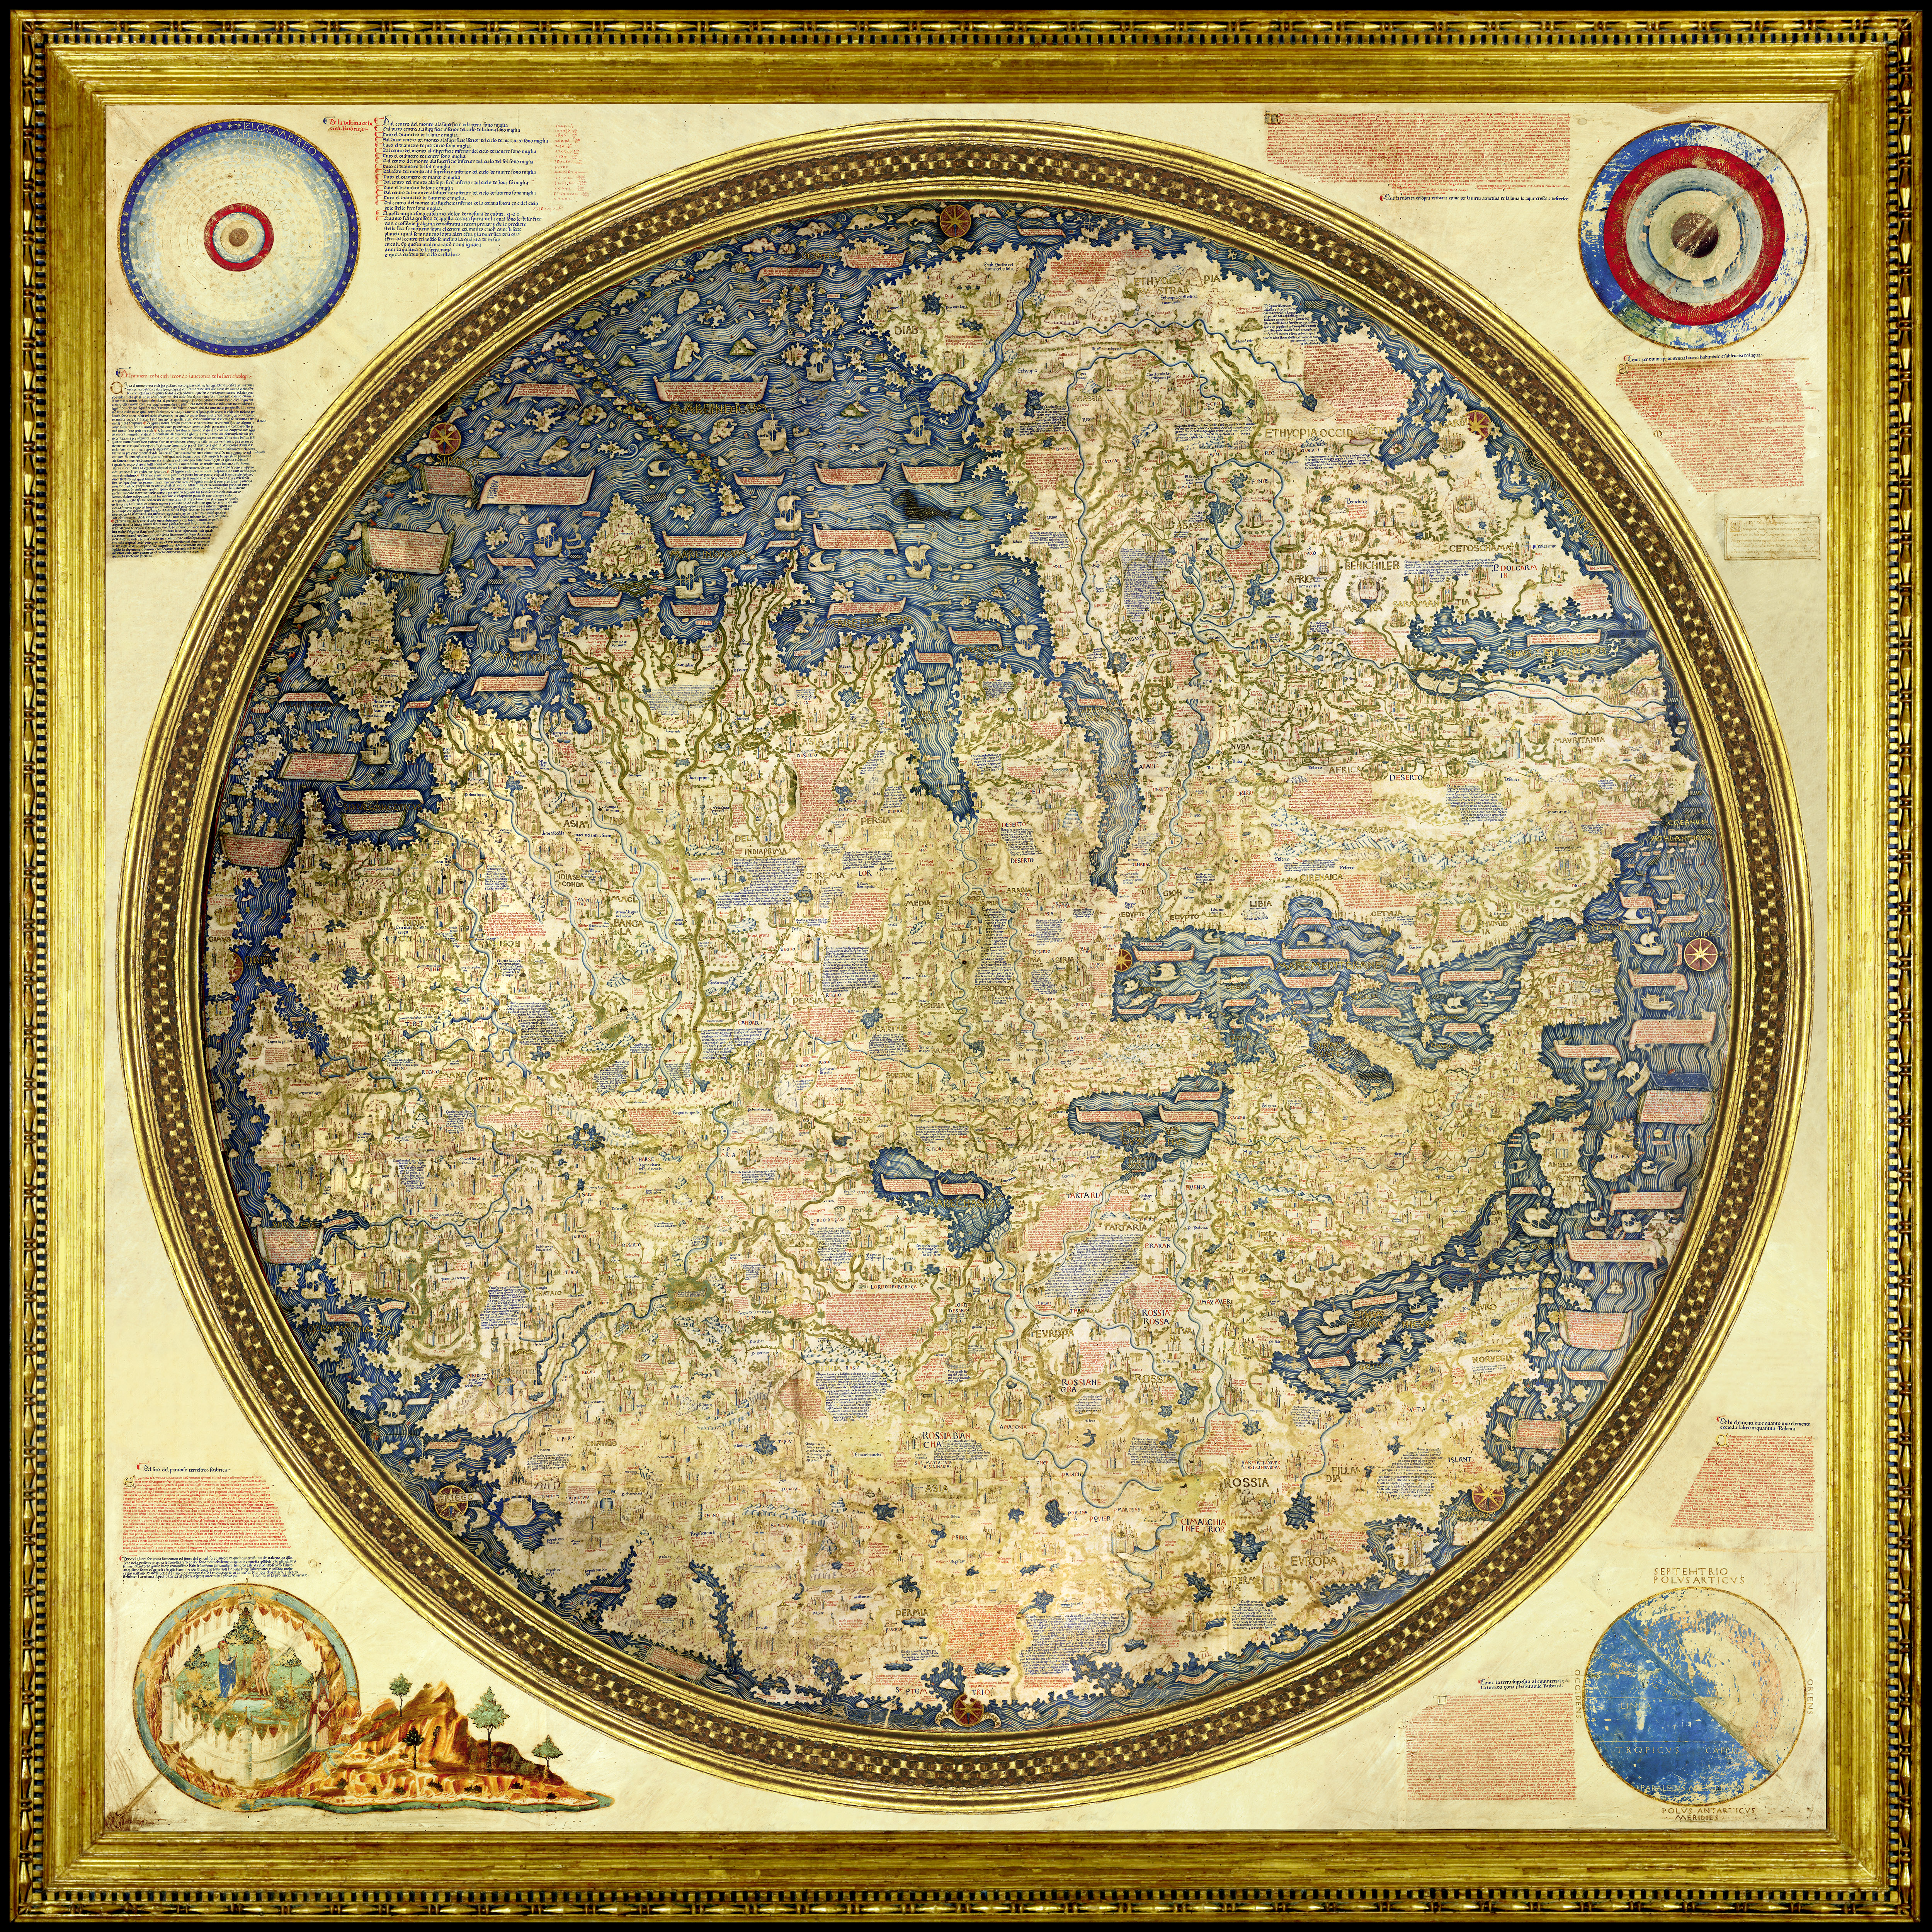
\includegraphics[keepaspectratio, height=\paperheight]{../img/fra_mauro_map}};
  \end{tikzpicture}
\end{frame}
% ----------------------------------------------------
\note{Mapa de Fra Mauro (c.~1450). Visión medieval del mundo: Europa, Asia, África conocidos pero con grandes lagunas. América no existe en el mapa.}

% ----------------------------------------------------
\begin{frame}
\frametitle{Un mundo fragmentado}
\centering

\begin{itemize}
  \item Sociedades aisladas, con escaso contacto entre sí
  \item Comercio a larga distancia existía, pero era caro y limitado
  \item No había un sistema político o económico global
\end{itemize}

\end{frame}
% ----------------------------------------------------
\note{Antes de 1500: la Ruta de la Seda existía, pero el comercio era limitado a bienes de lujo. Las grandes civilizaciones (China, Imperio Otomano, Europa) operaban de forma independiente. No había un ``sistema internacional''.}

% % ----------------------------------------------------
% \begin{frame}
% \frametitle{Para discutir}
% \centering

% \Large ¿Por qué creéis que fue \textbf{Europa} la que se expandió por el mundo y no, por ejemplo, China o el Imperio Otomano?

% \end{frame}
% % ----------------------------------------------------

% ----------------------------------------------------
\begin{frame}[plain]
  \begin{tikzpicture}[remember picture, overlay]
    \node[at = (current page.center), yshift = 0cm] (cover) {%
      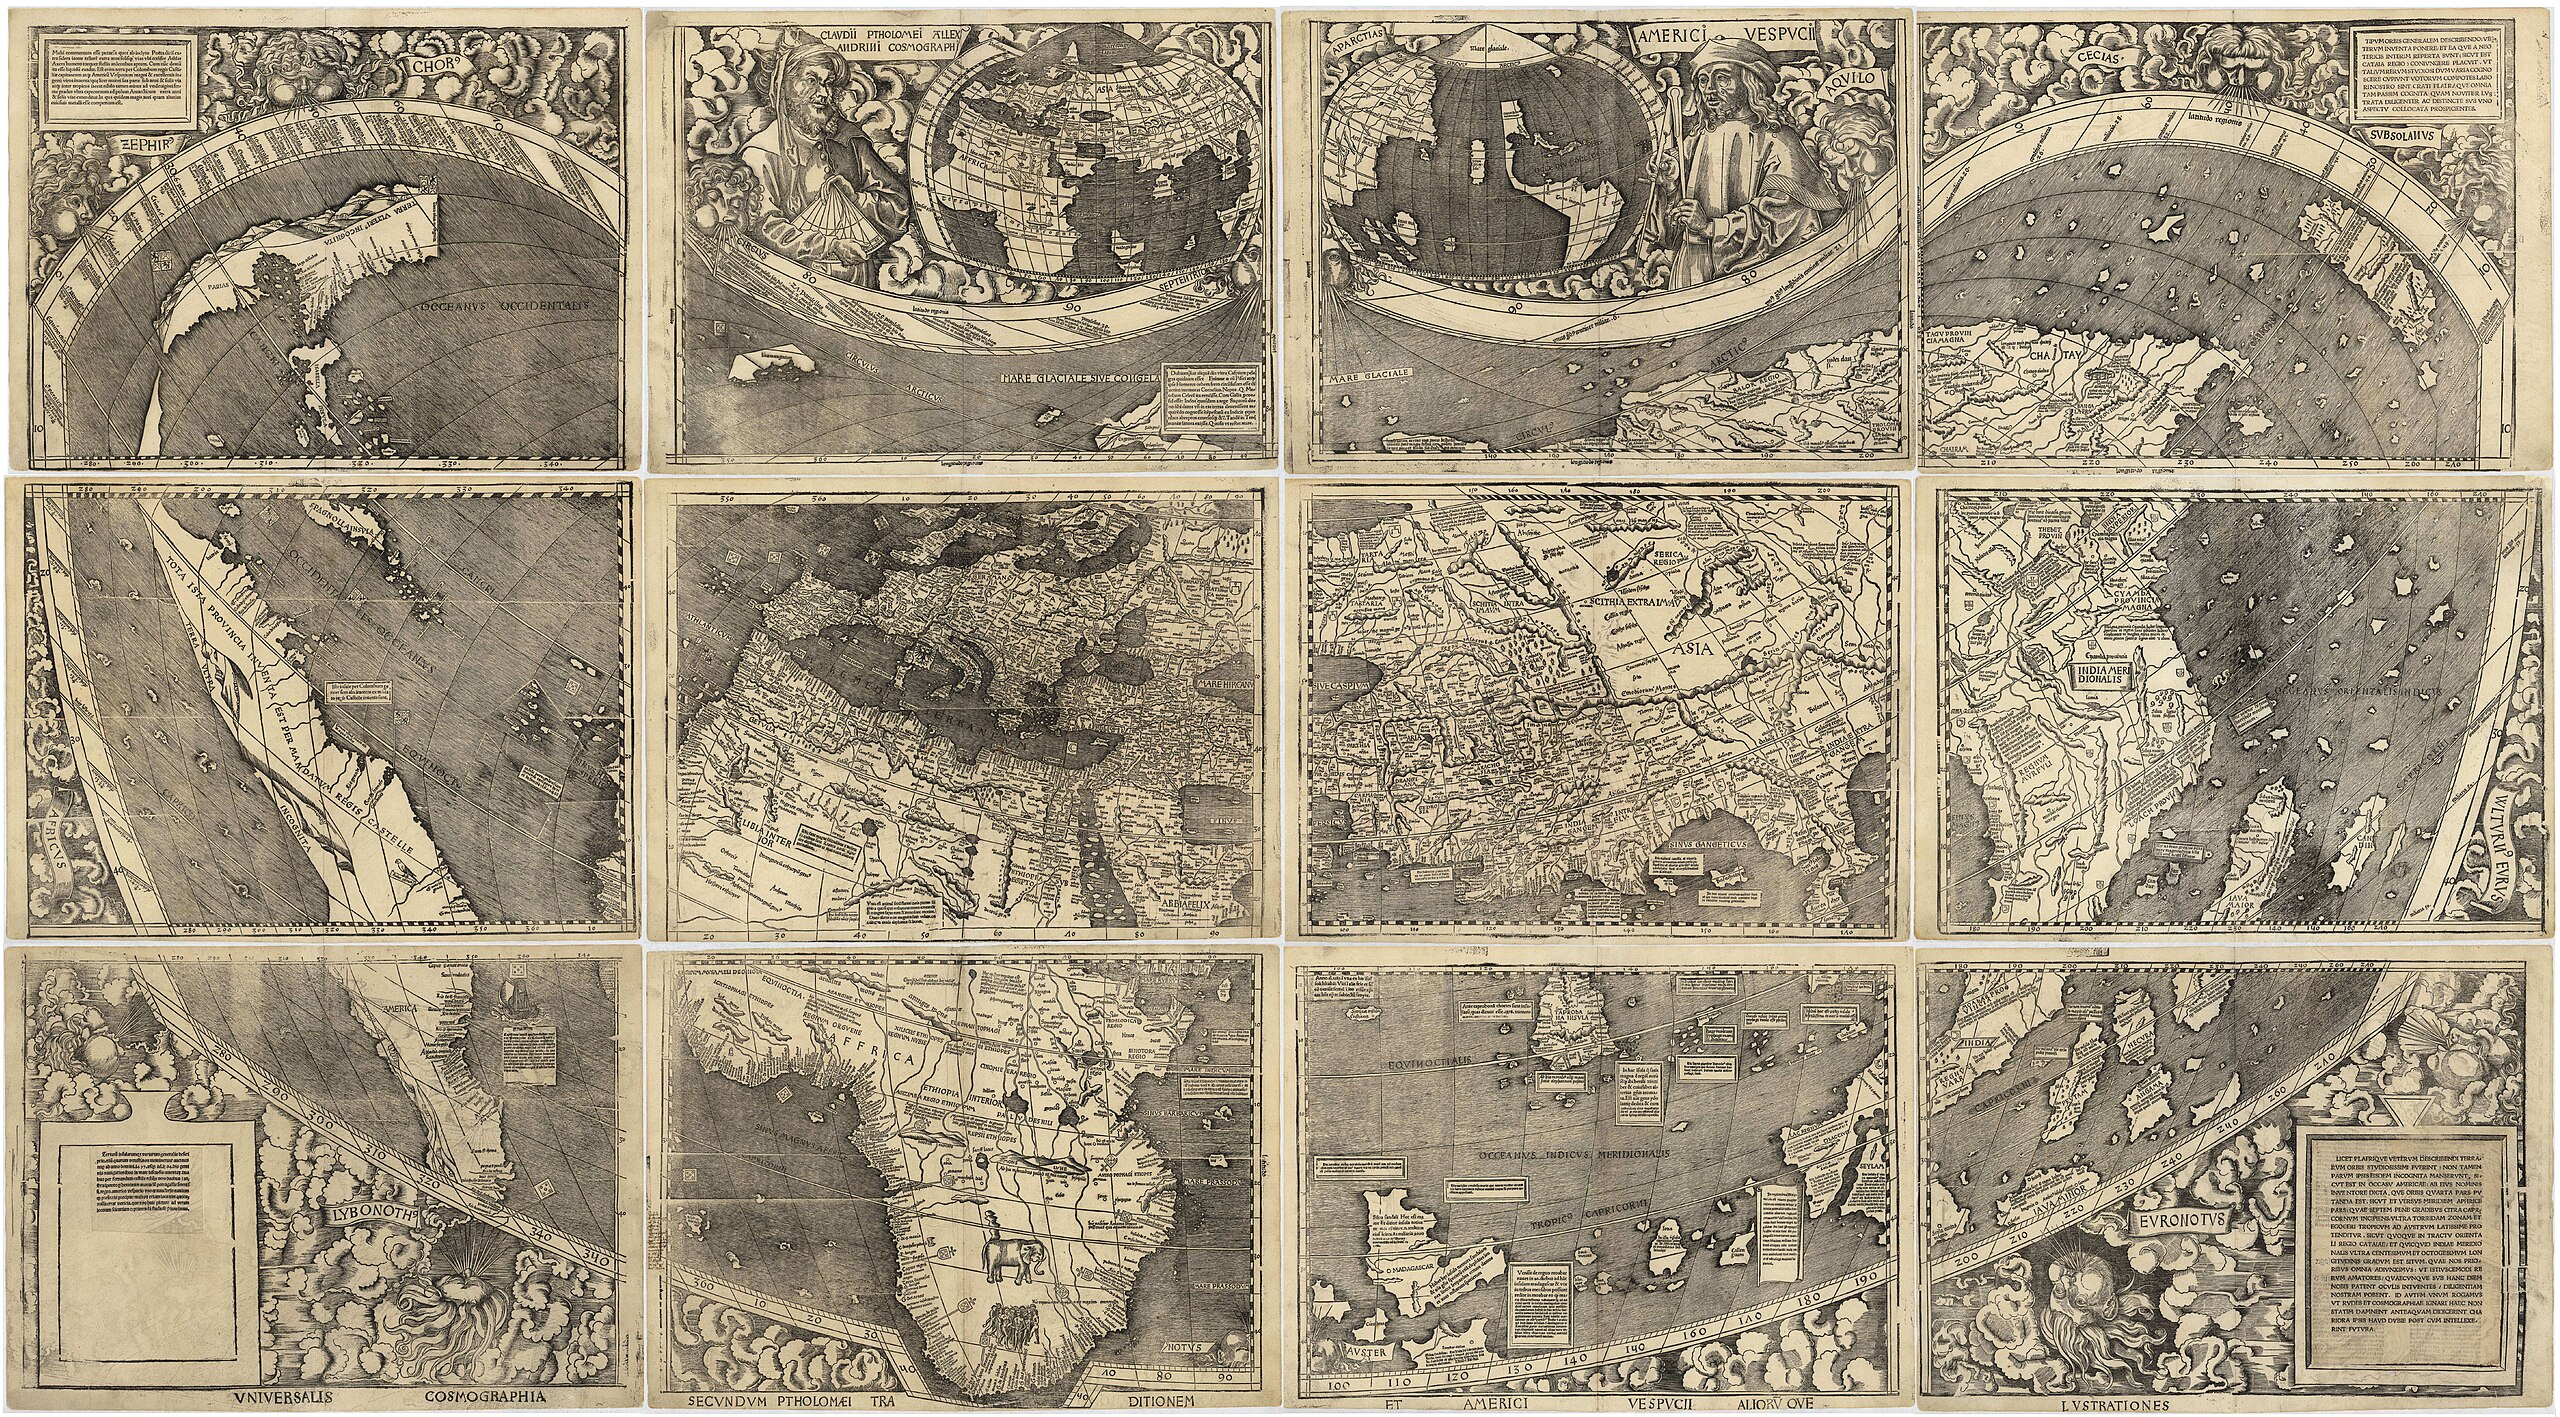
\includegraphics[keepaspectratio, height=\paperheight]{../img/waldseemuller_map}};
  \end{tikzpicture}
\end{frame}
% ----------------------------------------------------
\note{Mapa de Waldseemüller (1507). Primer mapa en usar el nombre ``América''. Marca el inicio de la era de exploración europea.}

% ----------------------------------------------------
\begin{frame}
\frametitle{Cinco siglos de política mundial}
\centering
\vspace{-5pt}
\begin{tikzpicture}

  % ---- Period bands (below the main line) ----
  \fill[accent!15] (-0.3, -0.15) rectangle (4.5, -0.55);
  \fill[yellow!20] (4.5, -0.15) rectangle (7.0, -0.55);
  \fill[red!12] (7.0, -0.15) rectangle (8.8, -0.55);
  \fill[accent!10] (8.8, -0.15) rectangle (10.3, -0.55);
  \fill[asher!8] (10.3, -0.15) rectangle (11.0, -0.55);

  % Period labels
  \node[font=\tiny\itshape, accent!80!black] at (2.1, -0.35) {Mercantilismo};
  \node[font=\tiny\itshape, yellow!40!black] at (5.75, -0.35) {Pax Britannica};
  \node[font=\tiny\itshape, red!60!black] at (7.9, -0.35) {Guerras mundiales};
  \node[font=\tiny\itshape, accent!60!black] at (9.55, -0.35) {Guerra Fría};

  % ---- Main timeline line ----
  \draw[thick, jet!50, ->] (-0.3, 0) -- (11.2, 0);

  % ---- Events (alternating TALL / SHORT ticks) ----

  % 1492 - TALL
  \fill[jet] (0.0, 0) circle (2pt);
  \draw[jet!30] (0.0, 0) -- (0.0, 2.0);
  \node[font=\tiny, align=center, anchor=south] at (0.0, 2.05) {%
    \textbf{1492}\\Desc. de\\América};

  % 1648 - SHORT
  \fill[jet] (1.7, 0) circle (2pt);
  \draw[jet!30] (1.7, 0) -- (1.7, 0.9);
  \node[font=\tiny, align=center, anchor=south] at (1.7, 0.95) {%
    \textbf{1648}\\Paz de\\Westfalia};

  % 1776 - TALL
  \fill[jet] (2.8, 0) circle (2pt);
  \draw[jet!30] (2.8, 0) -- (2.8, 2.0);
  \node[font=\tiny, align=center, anchor=south] at (2.8, 2.05) {%
    \textbf{1776}\\Revolución\\americana};

  % 1789 - SHORT
  \fill[jet] (3.5, 0) circle (2pt);
  \draw[jet!30] (3.5, 0) -- (3.5, 0.9);
  \node[font=\tiny, align=center, anchor=south] at (3.5, 0.95) {%
    \textbf{1789}\\Rev.\\Francesa};

  % 1815 - TALL
  \fill[jet] (4.5, 0) circle (2pt);
  \draw[jet!30] (4.5, 0) -- (4.5, 2.0);
  \node[font=\tiny, align=center, anchor=south] at (4.5, 2.05) {%
    \textbf{1815}\\Congreso\\de Viena};

  % ~1820 - SHORT
  \fill[jet] (5.3, 0) circle (2pt);
  \draw[jet!30] (5.3, 0) -- (5.3, 0.9);
  \node[font=\tiny, align=center, anchor=south] at (5.3, 0.95) {%
    \textbf{$\sim$1820}\\Indep.\\latinoam.};

  % 1884 - TALL
  \fill[jet] (6.3, 0) circle (2pt);
  \draw[jet!30] (6.3, 0) -- (6.3, 2.0);
  \node[font=\tiny, align=center, anchor=south] at (6.3, 2.05) {%
    \textbf{1884}\\Conf. de\\Berlín};

  % 1919 - SHORT
  \fill[jet] (7.5, 0) circle (2pt);
  \draw[jet!30] (7.5, 0) -- (7.5, 0.9);
  \node[font=\tiny, align=center, anchor=south] at (7.5, 0.95) {%
    \textbf{1919}\\Conf. de\\París};

  % 1945 - TALL
  \fill[jet] (8.8, 0) circle (2pt);
  \draw[jet!30] (8.8, 0) -- (8.8, 2.0);
  \node[font=\tiny, align=center, anchor=south] at (8.8, 2.05) {%
    \textbf{1945}\\Conf. de San\\Francisco};

  % 1989 - SHORT
  \fill[jet] (10.3, 0) circle (2pt);
  \draw[jet!30] (10.3, 0) -- (10.3, 0.9);
  \node[font=\tiny, align=center, anchor=south] at (10.3, 0.95) {%
    \textbf{1989}\\Caída del\\Muro de Berlín};

\end{tikzpicture}
\end{frame}
% ----------------------------------------------------
\note{Cronología general. Repasar brevemente cada era y evento. Usar como referencia visual para el resto de la clase. Los eventos marcan puntos de inflexión; las bandas de color muestran los períodos.}

% ----------------------------------------------------
\begin{frame}
\frametitle{La expansión europea después de 1492}
\centering

\begin{itemize}
  \item España, Portugal, Inglaterra, Francia, Países Bajos
  \item Conquista, colonización, comercio
  \item Hacia 1700, Europa controla gran parte del mundo
\end{itemize}

\end{frame}
% ----------------------------------------------------
\note{España y Portugal primero (Tratado de Tordesillas, 1494). Luego Inglaterra, Francia y Países Bajos. La competencia entre potencias europeas es un motor clave. Consecuencias devastadoras para las poblaciones locales.}

% ----------------------------------------------------
\begin{frame}[plain]
  \begin{tikzpicture}[remember picture, overlay]
    \node[at = (current page.center), yshift = 0cm] (cover) {%
      \includegraphics[keepaspectratio, height=.85\paperheight]{
      ../img/mercantilism_map_world}};
  \end{tikzpicture}
\end{frame}
% ----------------------------------------------------
\note{Mapa de rutas comerciales mercantilistas. Mostrar cómo el comercio colonial conectaba Europa con el resto del mundo.}

% ----------------------------------------------------
\begin{frame}
\frametitle{El mercantilismo}
\centering

\begin{itemize}
  \item El poder militar genera riqueza; la riqueza financia la guerra
  \item Monopolios comerciales: las colonias sirven a la metrópoli
  \item \textit{``Foreign trade produces riches, riches power, power preserves our trade and religion''}
\end{itemize}

\end{frame}
% ----------------------------------------------------
\note{Lógica circular: riqueza $\rightarrow$ poder $\rightarrow$ riqueza. Ejemplos: Compañía de las Indias Orientales (holandesa y británica), monopolio español sobre plata americana. Coste para las colonias: caso del tabaco en Virginia (precios artificialmente bajos).}

% ----------------------------------------------------
\begin{frame}[plain]
  \begin{tikzpicture}[remember picture, overlay]
    \node[at = (current page.center), yshift = 0cm] (cover) {%
      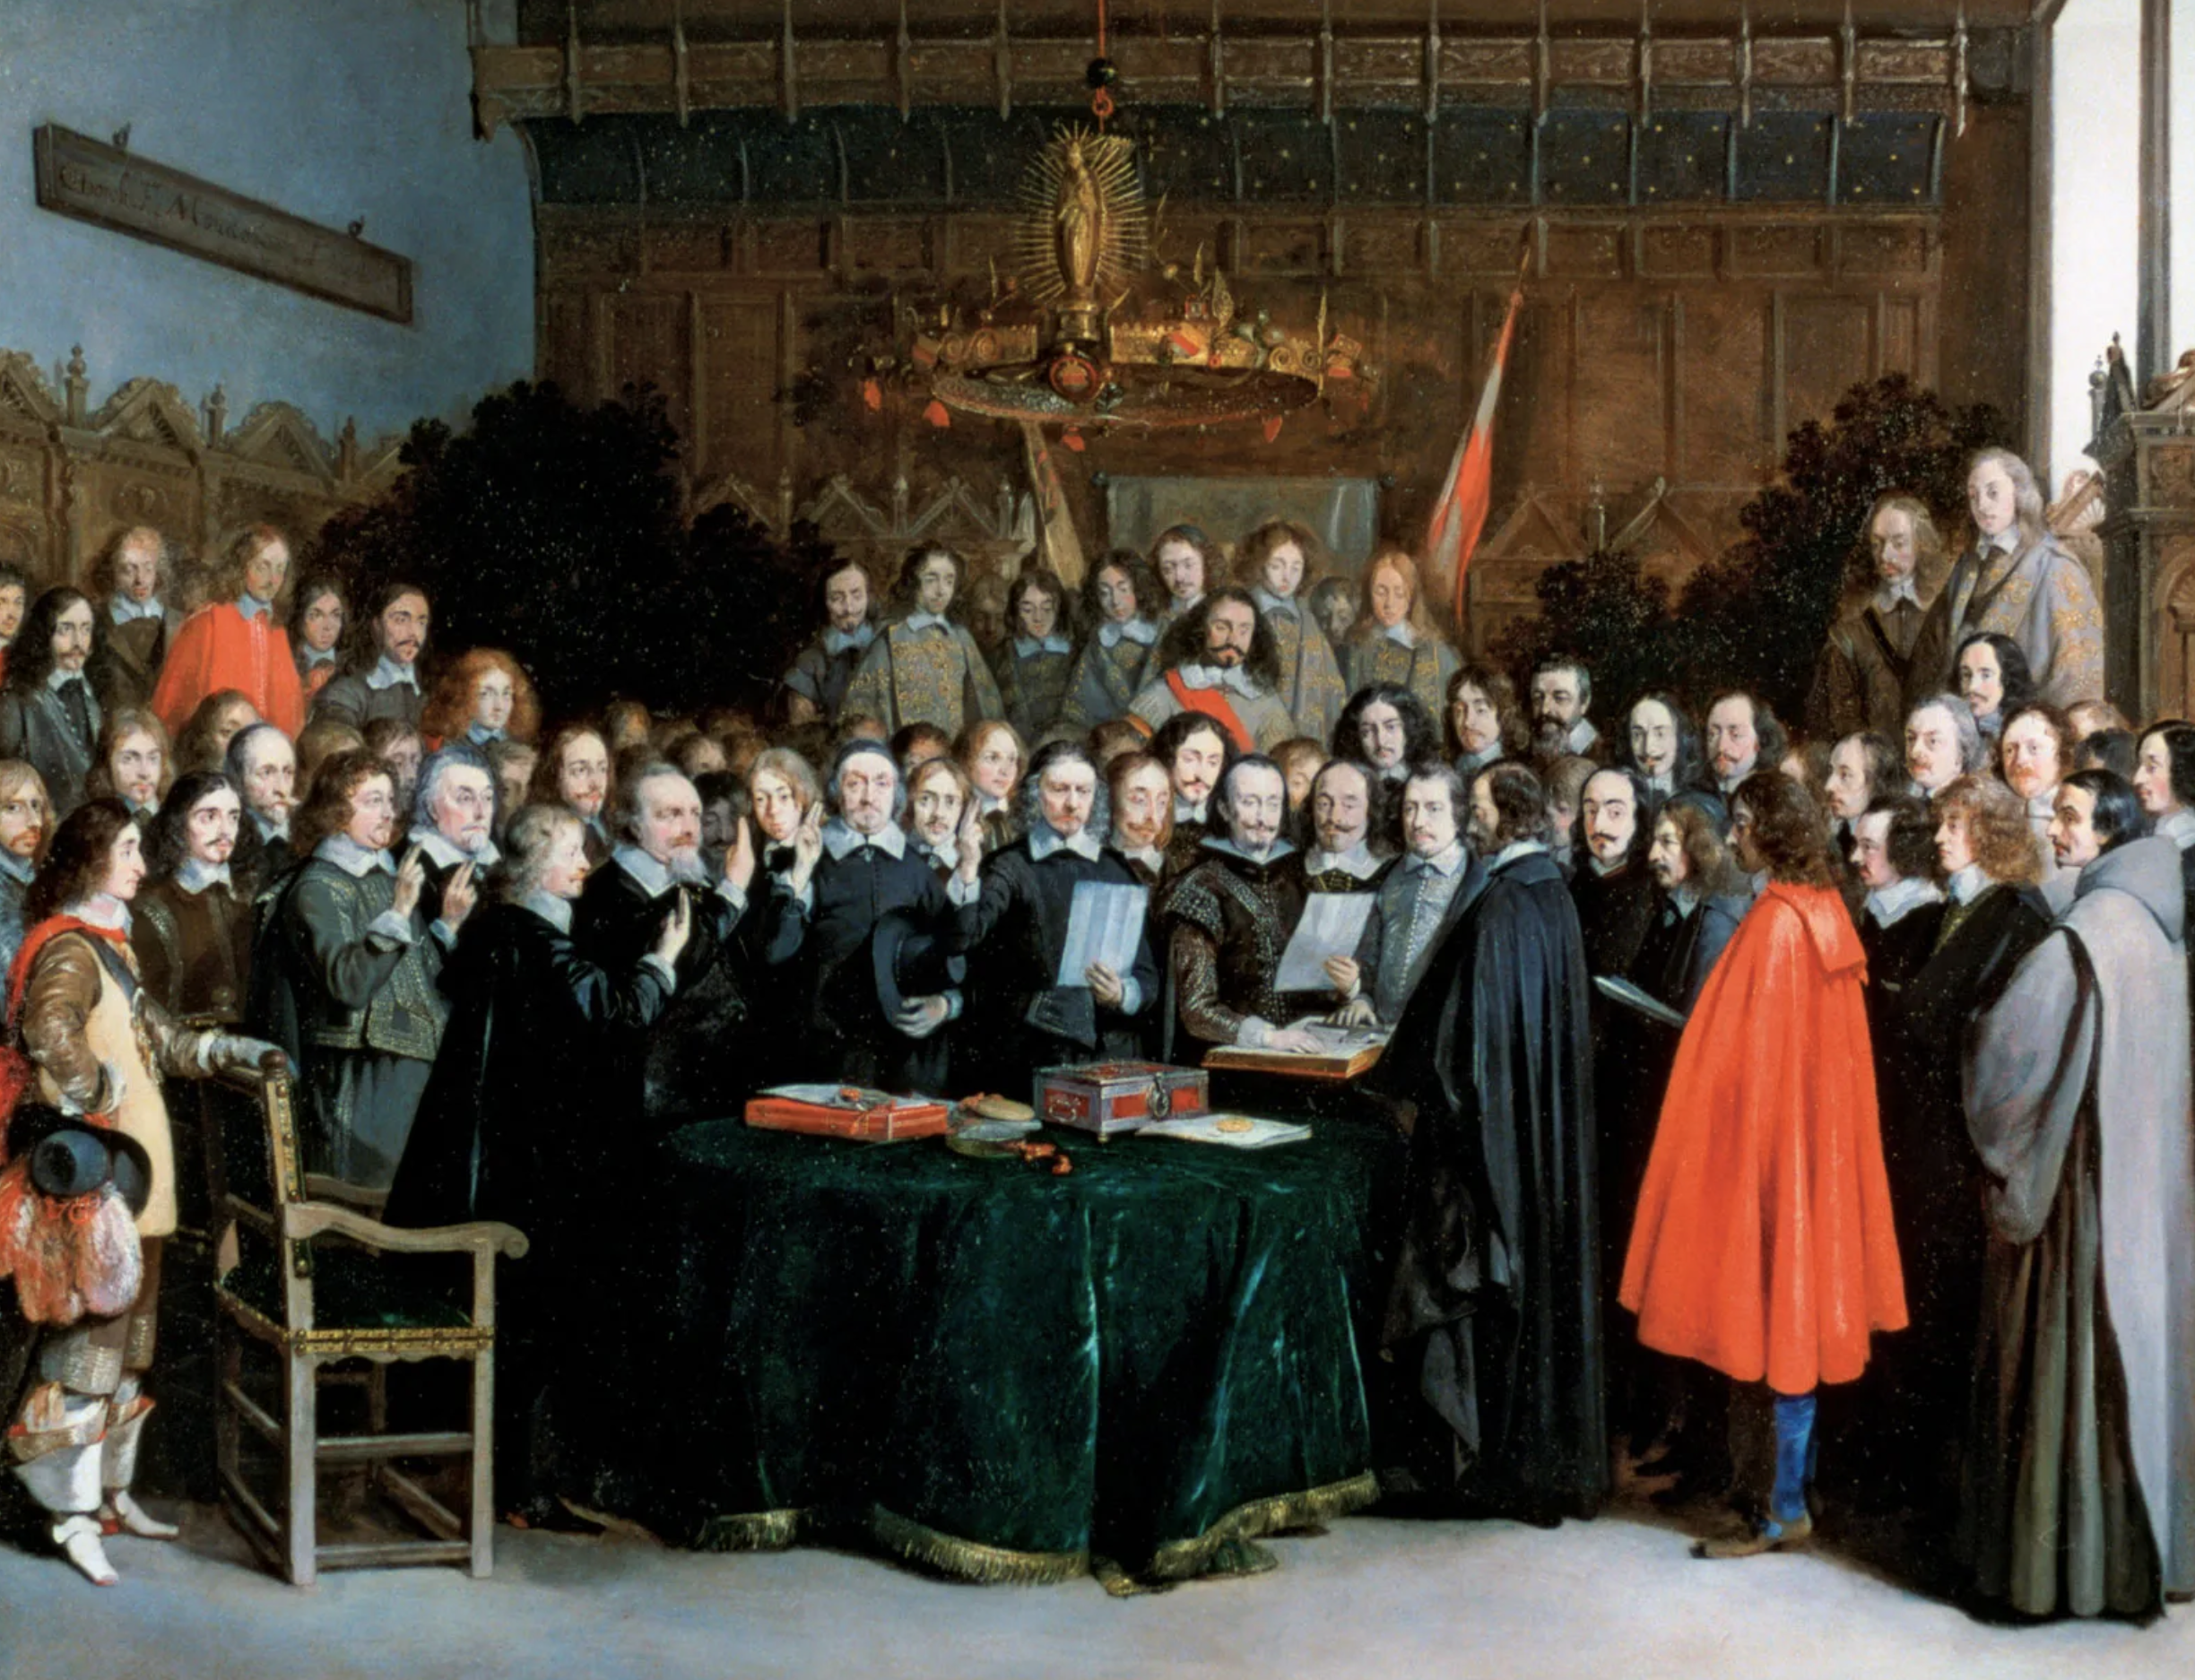
\includegraphics[keepaspectratio, height=\paperheight]{../img/peace_of_westphalia}};
  \end{tikzpicture}
\end{frame}
% ----------------------------------------------------
\note{Cuadro de la firma de la Paz de Westfalia (1648). Fin de la Guerra de los Treinta Años.}

% ----------------------------------------------------
\begin{frame}
\frametitle{La Paz de Westfalia (1648)}
\centering

\begin{itemize}
  \item Fin de la Guerra de los Treinta Años
  \item Principio de \textbf{soberanía}: cada Estado es supremo dentro de sus fronteras
  \item Origen del sistema moderno de Estados
\end{itemize}

\end{frame}
% ----------------------------------------------------
\note{Concepto clave: soberanía y no intervención. Es el fundamento del sistema internacional moderno. Discutir: ¿sigue vigente hoy este principio? Ejemplos de tensión: intervenciones humanitarias, Ucrania, Kosovo.}


% ====================================================
\section{La Pax Britannica (1815--1914)}
% ====================================================

% ----------------------------------------------------
\begin{frame}[plain]
  \begin{tikzpicture}[remember picture, overlay]
    \node[at = (current page.center), yshift = 0cm] (cover) {%
      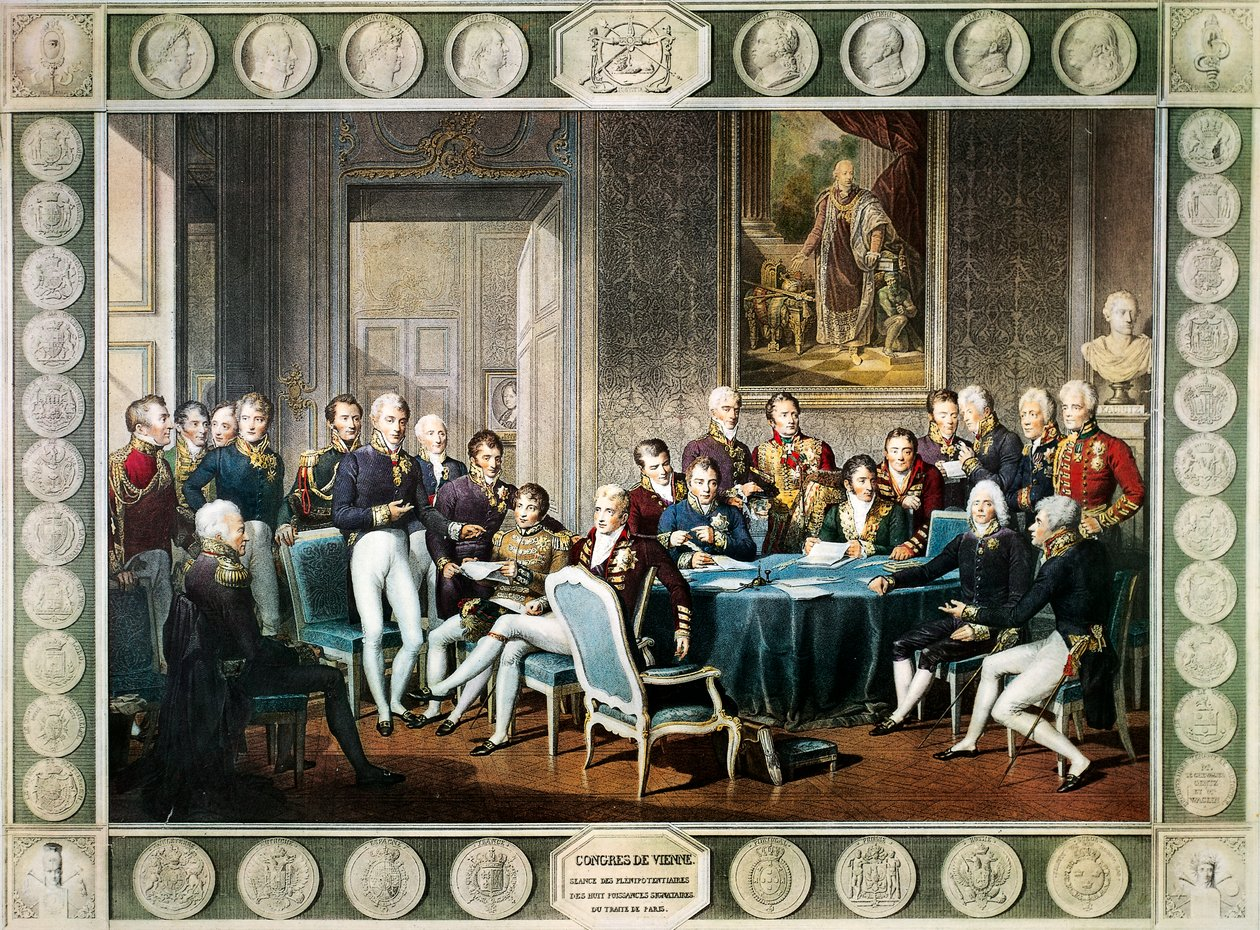
\includegraphics[keepaspectratio, height=\paperheight]{../img/congress_vienna}};
  \end{tikzpicture}
\end{frame}
% ----------------------------------------------------
\note{Congreso de Viena (1814--15). Rediseño del mapa de Europa tras la derrota de Napoleón. Inicio de un siglo de relativa estabilidad.}

% ----------------------------------------------------
\begin{frame}
\frametitle{Un siglo de relativa paz}
\centering

\begin{itemize}
  \item Tras las guerras napoleónicas, las grandes potencias cooperan
  \item Hegemonía británica: equilibrio de poder en Europa
  \item Crecimiento económico sin precedentes
\end{itemize}

\end{frame}
% ----------------------------------------------------
\note{Pax Britannica: hegemonía naval y económica de Gran Bretaña estabiliza el sistema. Concierto de Europa: las potencias se consultan. El PIB per cápita se cuadruplica entre 1815 y 1914.}

% ----------------------------------------------------
\begin{frame}[plain]
  \begin{tikzpicture}[remember picture, overlay]
    \node[at = (current page.center), yshift = 0cm] (cover) {%
      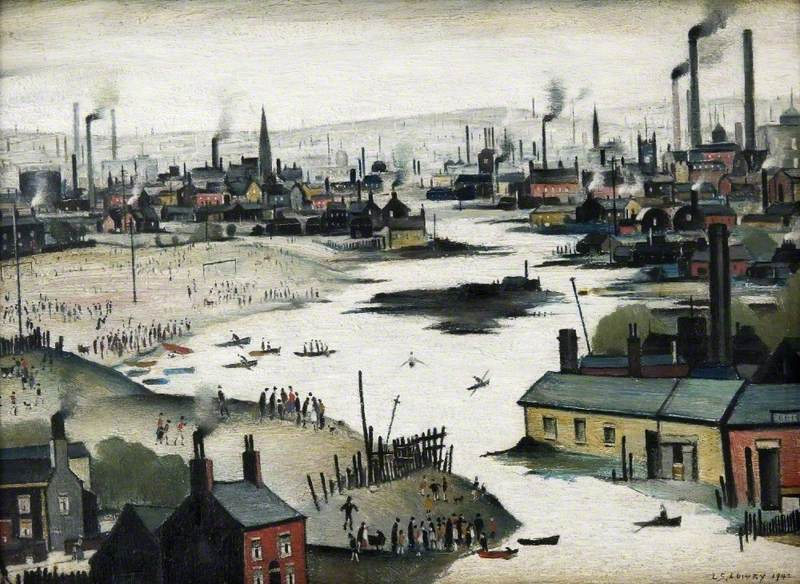
\includegraphics[keepaspectratio, height=\paperheight]{../img/industrial_revolution}};
  \end{tikzpicture}
\end{frame}
% ----------------------------------------------------
\note{Imagen de la Revolución Industrial. Transformación radical de la producción y el transporte.}

% ----------------------------------------------------
\begin{frame}
\frametitle{La primera globalización}
\centering

\begin{itemize}
  \item Revolución Industrial $\rightarrow$ libre comercio
  \item Patrón oro: estabilidad monetaria internacional
  \item Migraciones masivas: 50 millones dejan Europa antes de 1914
\end{itemize}

\end{frame}
% ----------------------------------------------------
\note{Primera globalización real. Gran Bretaña abandona el mercantilismo (derogación de las Corn Laws, 1846). El patrón oro facilita comercio e inversión. 50 millones de europeos emigran. Comparar con la globalización actual: ¿similitudes y diferencias?}

% ----------------------------------------------------
\begin{frame}[plain]
  \begin{tikzpicture}[remember picture, overlay]
    \node[at = (current page.center), yshift = 0cm] (cover) {%
      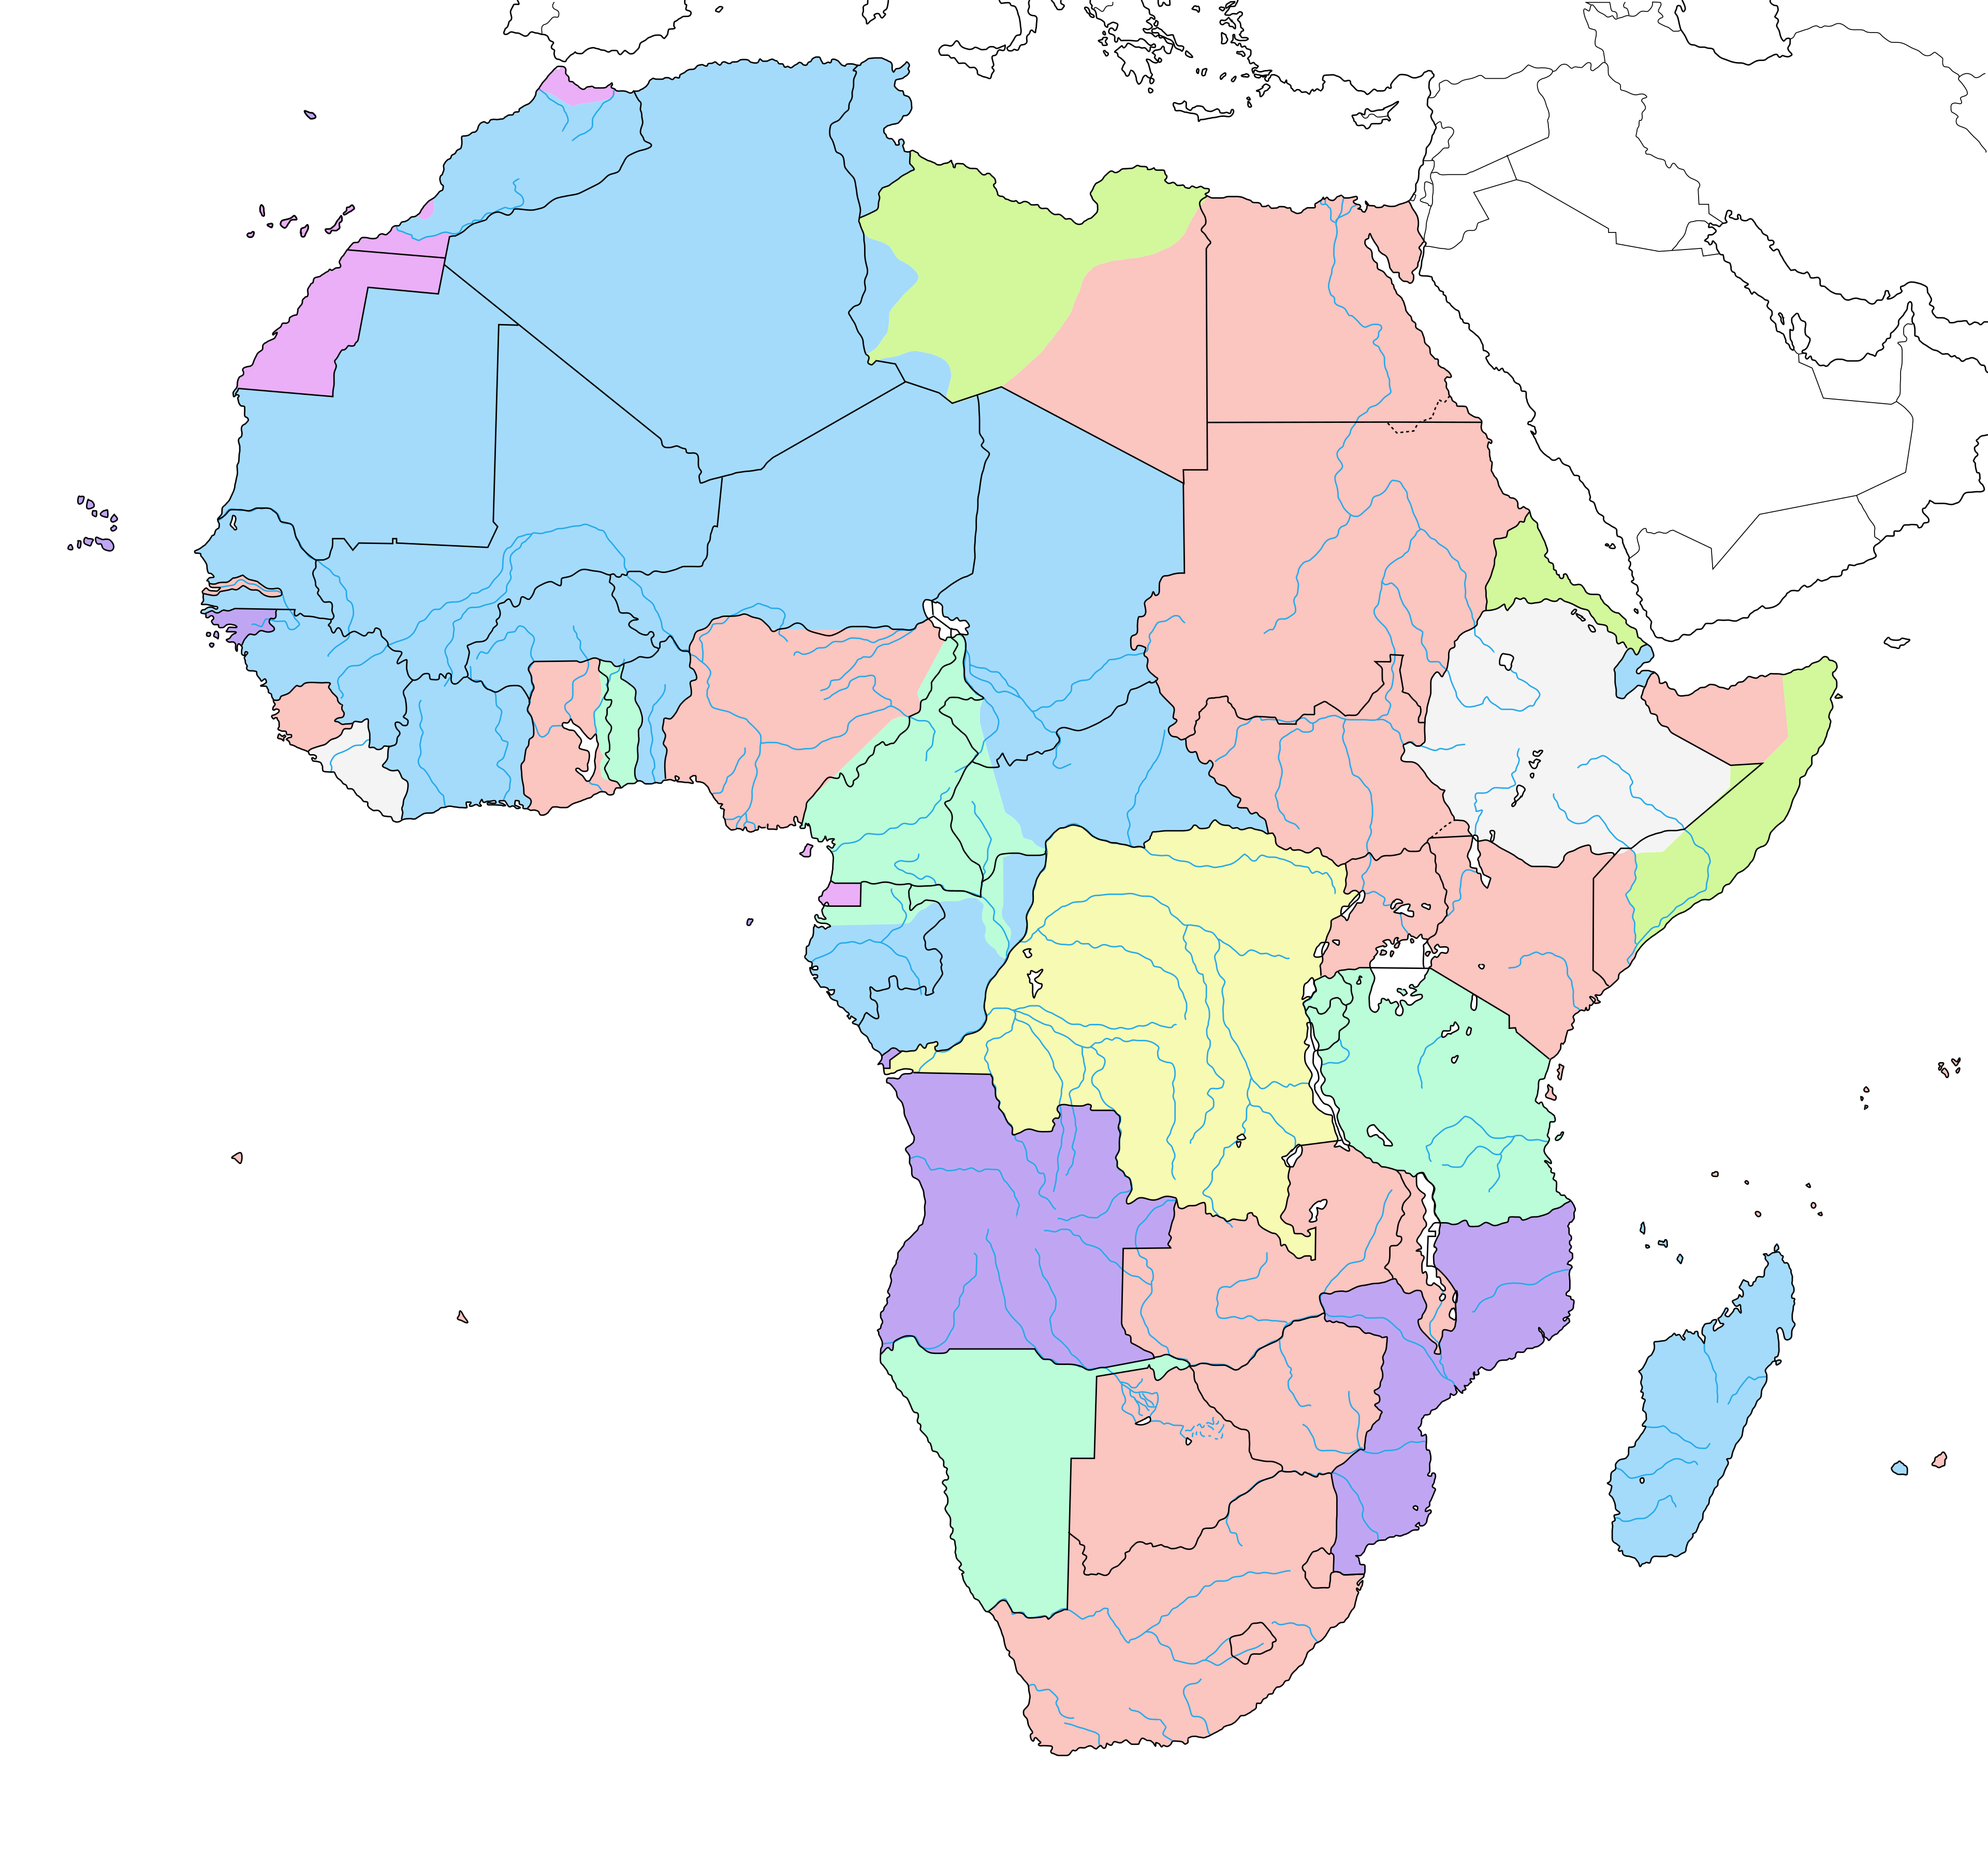
\includegraphics[keepaspectratio, height=\paperheight]{../img/scramble_africa}};
  \end{tikzpicture}
\end{frame}
% ----------------------------------------------------
\note{Mapa del reparto colonial de África (c.~1914). Casi todo el continente colonizado excepto Etiopía y Liberia.}

% ----------------------------------------------------
\begin{frame}
\frametitle{La otra cara: el imperialismo colonial}
\centering

\begin{itemize}
  \item Paz en Europa, pero expansión militar en África y Asia
  \item Hacia 1890, casi toda África está colonizada
  \item Las potencias compiten por territorios y recursos
\end{itemize}

\end{frame}
% ----------------------------------------------------
\note{La Pax Britannica era paz entre europeos, no paz global. Conferencia de Berlín (1884): reparto de África sin consultar a los africanos. Nuevas potencias (Alemania, Italia, Japón, EE.UU.) quieren su parte del pastel colonial.}

% % ----------------------------------------------------
% \begin{frame}
% \frametitle{Para discutir}
% \centering

% \Large ¿Se puede hablar de \textbf{paz} y \textbf{prosperidad} en un período de colonialismo masivo?

% \end{frame}
% % ----------------------------------------------------


% ====================================================
\section{Los años de guerras (1914--1945)}
% ====================================================

% ----------------------------------------------------
\begin{frame}[plain]
  \begin{tikzpicture}[remember picture, overlay]
    \node[at = (current page.center), yshift = 0cm] (cover) {%
      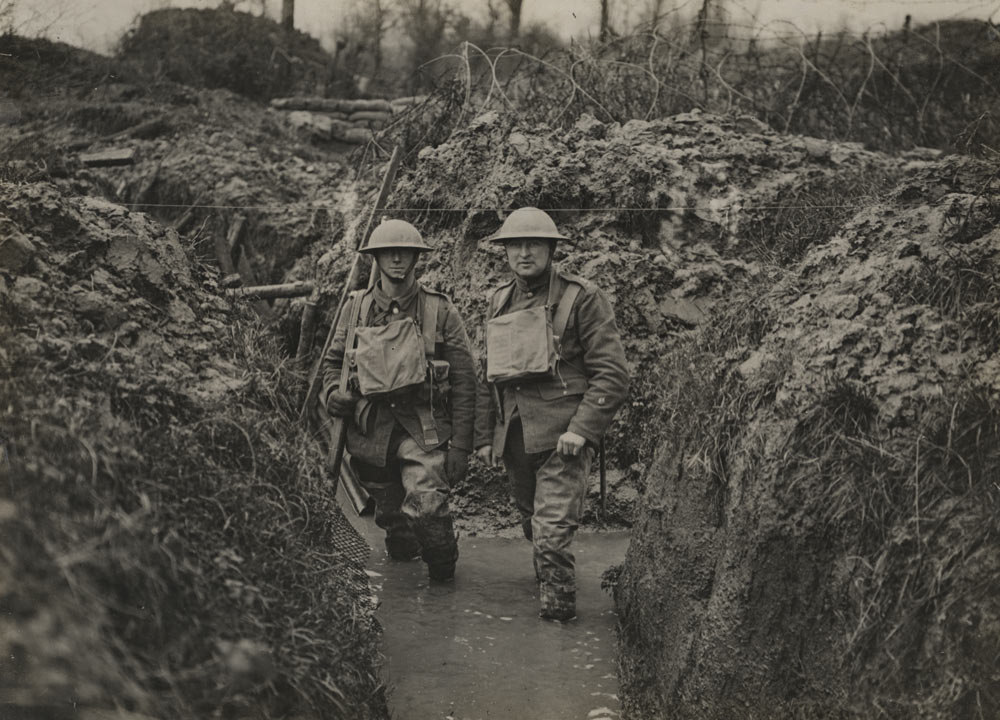
\includegraphics[keepaspectratio, height=\paperheight]{../img/wwi_trenches}};
  \end{tikzpicture}
\end{frame}
% ----------------------------------------------------
\note{Fotografía de trincheras de la Primera Guerra Mundial. Guerra de posiciones, enormes pérdidas humanas.}

% ----------------------------------------------------
\begin{frame}
\frametitle{La Primera Guerra Mundial}
\centering

\begin{itemize}
  \item 15 millones de muertos
  \item Colapso de cuatro imperios
  \item EE.UU. emerge como futura potencia decisiva
\end{itemize}

\end{frame}
% ----------------------------------------------------
\note{Imperios que colapsan: otomano, austrohúngaro, ruso, alemán. Nuevos Estados inestables en Europa central y oriental. EE.UU. entra en 1917 y es decisivo, pero luego se retira (no entra en la Sociedad de Naciones). Tratado de Versailles: reparaciones y resentimiento alemán.}

% ----------------------------------------------------
\begin{frame}[plain]
  \begin{tikzpicture}[remember picture, overlay]
    \node[at = (current page.center), yshift = 0cm] (cover) {%
      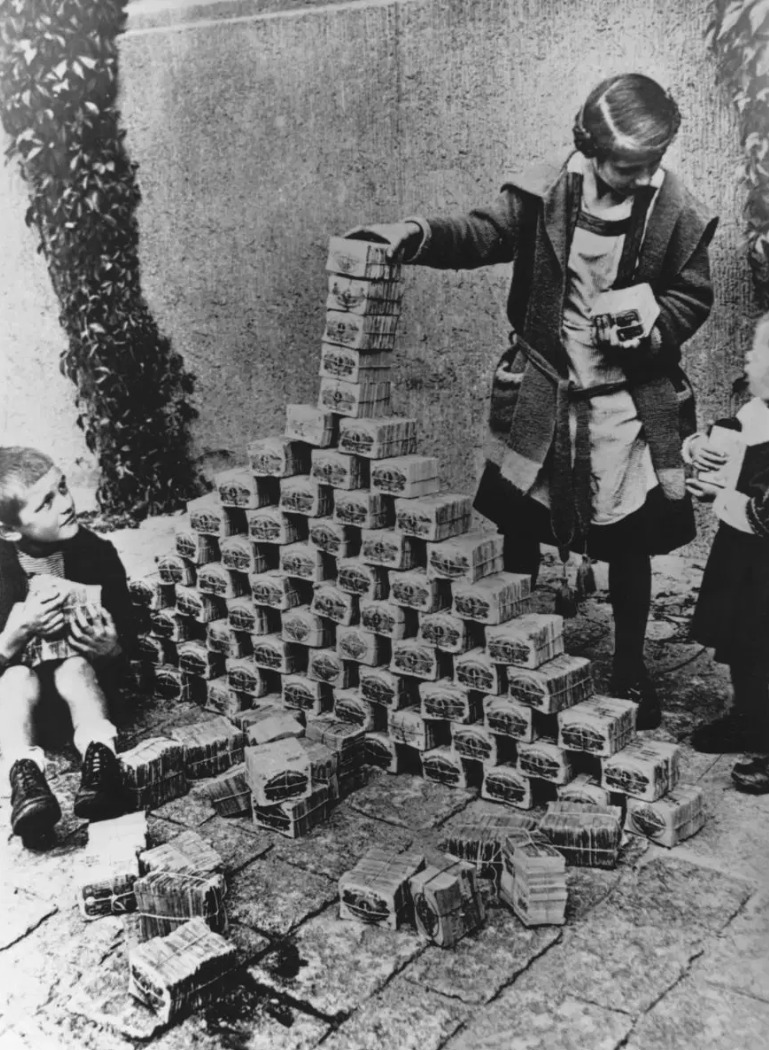
\includegraphics[keepaspectratio, height=\paperheight]{../img/weimar_hyperinflation}};
  \end{tikzpicture}
\end{frame}
% ----------------------------------------------------
\note{Hiperinflación en Alemania (1923): niños jugando con fajos de billetes. 1 dólar = 4,2 billones de marcos. La clase media queda arruinada, lo que alimenta el extremismo político.}

% % ----------------------------------------------------
% \begin{frame}
% \frametitle{Entreguerras: la espiral hacia el desastre}
% \centering

% \begin{itemize}
%   \item Hiperinflación, Gran Depresión, desempleo masivo
%   \item Ascenso del fascismo y del comunismo
%   \item Polarización política extrema
% \end{itemize}

% \end{frame}
% % ----------------------------------------------------

% ----------------------------------------------------
\begin{frame}[plain]
  \begin{tikzpicture}[remember picture, overlay]
    \node[at = (current page.center), yshift = 0cm] (cover) {%
      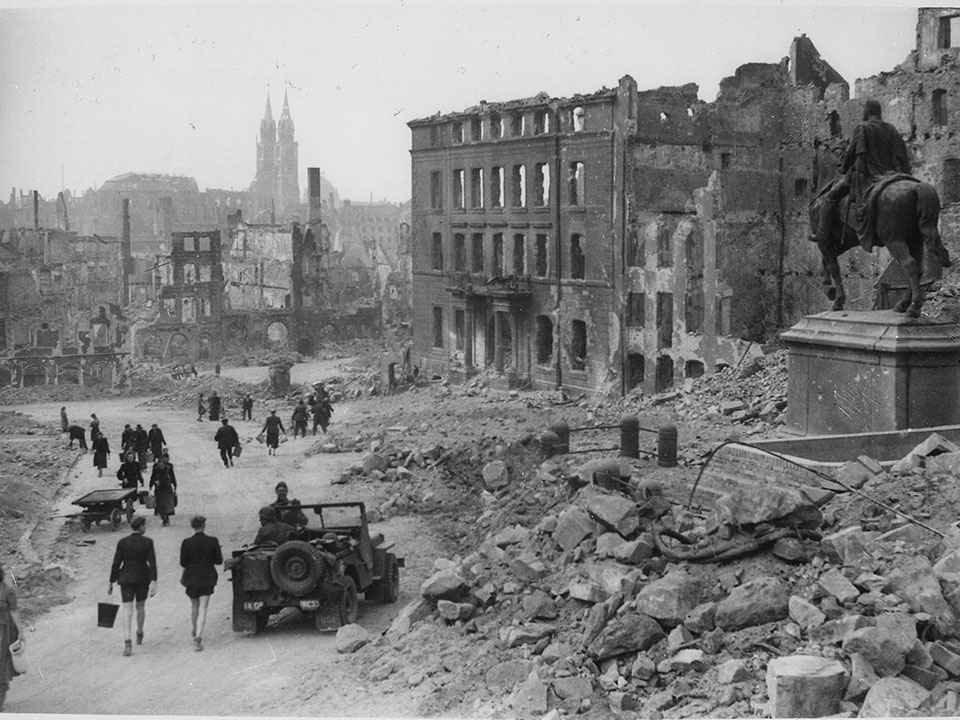
\includegraphics[keepaspectratio, height=\paperheight]{../img/wwii_destruction}};
  \end{tikzpicture}
\end{frame}
% ----------------------------------------------------
\note{Imagen de destrucción de la Segunda Guerra Mundial. 55 millones de muertos. Holocausto. Bombas nucleares en Hiroshima y Nagasaki.}

% % ----------------------------------------------------
% \begin{frame}
% \frametitle{La Segunda Guerra Mundial}
% \centering

% \begin{itemize}
%   \item 55 millones de muertos, incluyendo el Holocausto
%   \item Europa y Japón en ruinas
%   \item Uso de armas nucleares: Hiroshima y Nagasaki
% \end{itemize}

% \end{frame}
% % ----------------------------------------------------

% ----------------------------------------------------
\begin{frame}
\frametitle{1945}
\centering

\begin{itemize}
  \item Se crea la ONU en la conferencia de San Francisco
  \begin{itemize}
    \item Le siguen todas las agencias: FAO, WHO (OMS), ILO (OIT, que ya existía), UNESCO, IMF (FMI)
  \end{itemize}
  \item Nunca antes hubo un sistema internacional tan desarrollado
  \item Gran influencia durante los primeros años
\end{itemize}

\end{frame}
% ----------------------------------------------------
\note{1945: momento fundacional del orden internacional actual. ONU, Bretton Woods (FMI, Banco Mundial), GATT. El sistema refleja los intereses de los vencedores (especialmente EE.UU.). Consejo de Seguridad con veto de las 5 potencias.}


% ====================================================
\section{La Guerra Fría}
% ====================================================

% ----------------------------------------------------
\begin{frame}[plain]
  \begin{tikzpicture}[remember picture, overlay]
    \node[at = (current page.center), yshift = 0cm] (cover) {%
      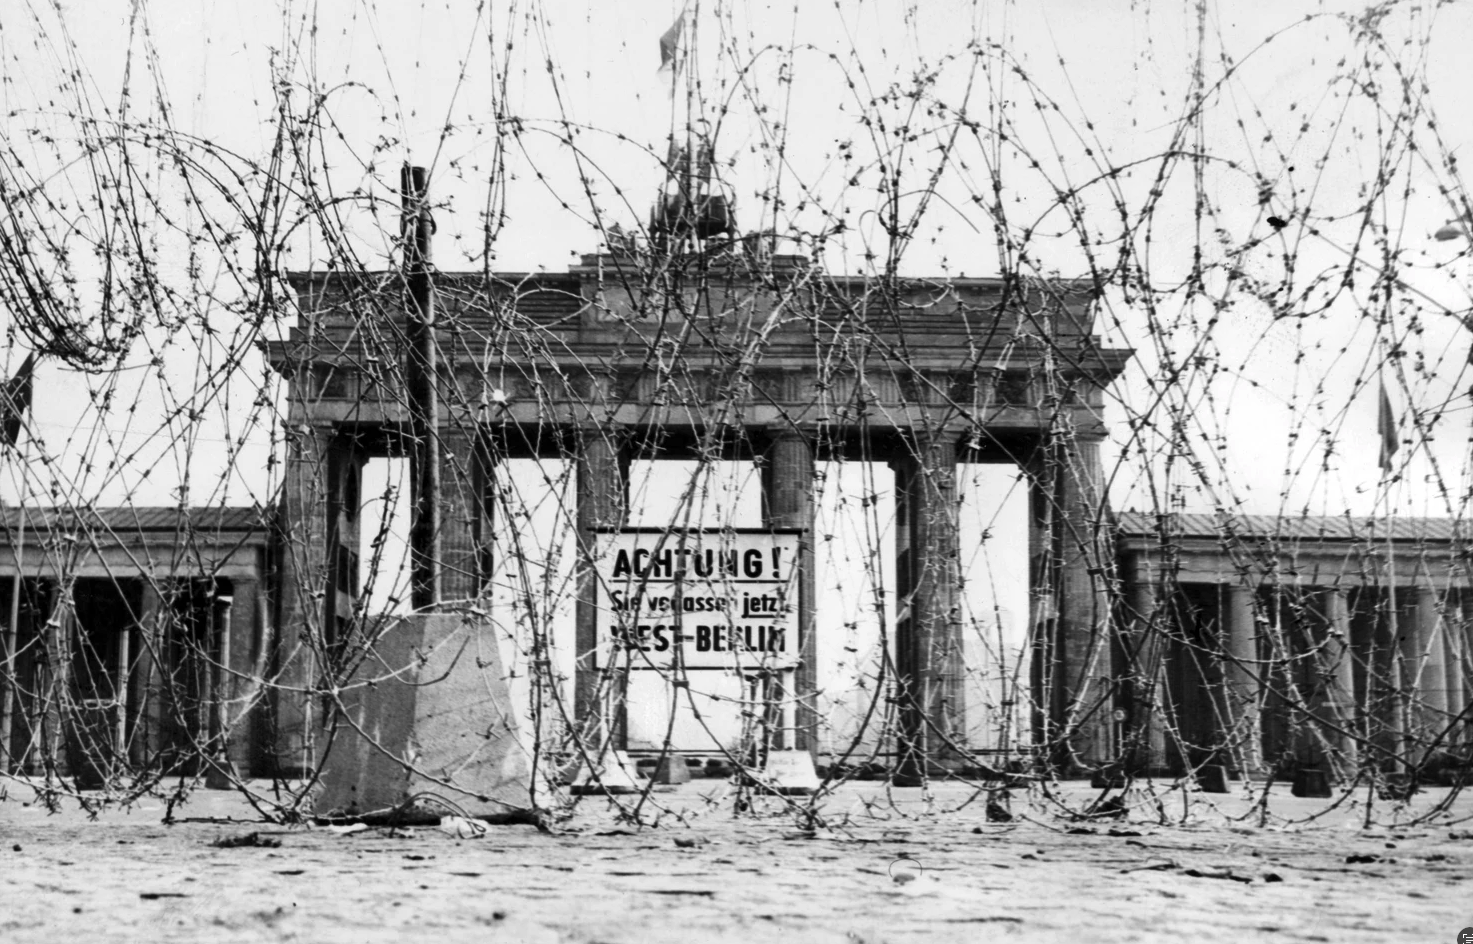
\includegraphics[keepaspectratio, height=\paperheight]{../img/berlin_wall}};
  \end{tikzpicture}
\end{frame}
% ----------------------------------------------------
\note{El Muro de Berlín: símbolo físico de la división del mundo en dos bloques.}

% ----------------------------------------------------
\begin{frame}
\frametitle{Un mundo dividido en dos}
\centering

\begin{itemize}
  \item EE.UU. vs. URSS: capitalismo vs. comunismo
  \item OTAN y Pacto de Varsovia
  \item Disuasión nuclear: destrucción mutua asegurada
\end{itemize}

\end{frame}
% ----------------------------------------------------
\note{Dos modelos económicos y políticos enfrentados. OTAN (1949) vs. Pacto de Varsovia (1955). MAD (Mutual Assured Destruction): la guerra nuclear es demasiado costosa para ambos lados. Bloque occidental: Plan Marshall, reconstrucción, Bretton Woods. Bloque oriental: planificación central, COMECON.}

% ----------------------------------------------------
\begin{frame}[plain]
  \begin{tikzpicture}[remember picture, overlay]
    \node[at = (current page.center), yshift = 0cm] (cover) {%
      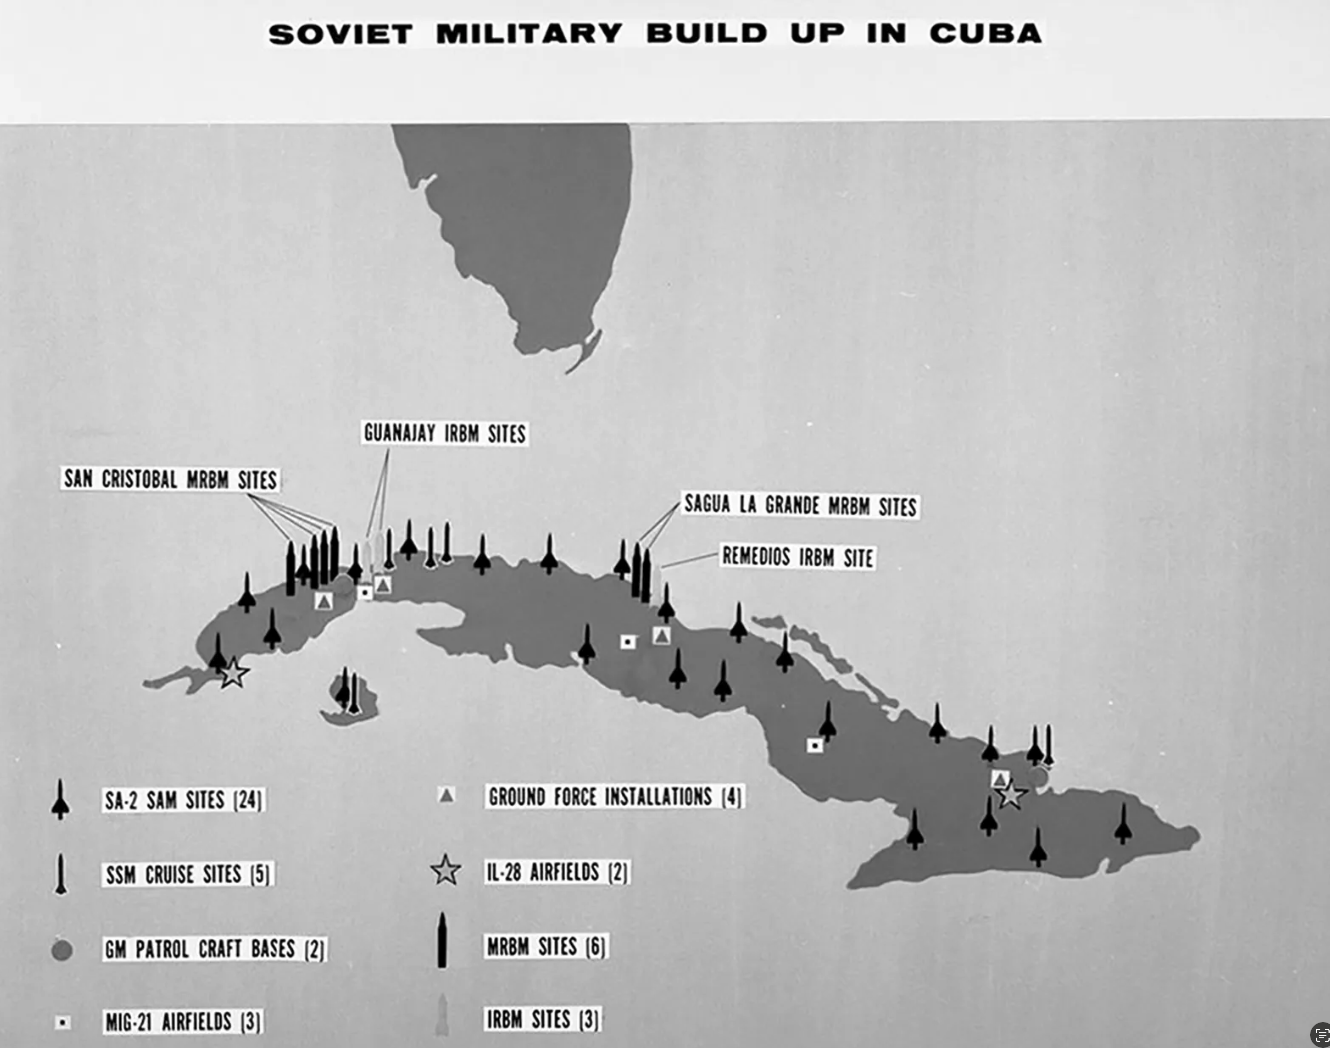
\includegraphics[keepaspectratio, height=\paperheight]{../img/cuban_missile_crisis}};
  \end{tikzpicture}
\end{frame}
% ----------------------------------------------------
\note{Crisis de los misiles de Cuba (1962). Foto de reconocimiento aéreo o de Kennedy. El momento más cercano a una guerra nuclear. Se resolvió con diplomacia secreta.}

% ----------------------------------------------------
\begin{frame}
\frametitle{Guerras proxy y descolonización}
\centering

\begin{itemize}
  \item Las superpotencias compiten en el ``Tercer Mundo''
  \item Guerras en Corea, Vietnam, Afganistán...
  \item Descolonización masiva en África y Asia
\end{itemize}

\end{frame}
% ----------------------------------------------------
\note{No hubo guerra directa entre EE.UU. y URSS, pero sí guerras proxy devastadoras. Corea (1950--53), Vietnam (1955--75), Afganistán (1979--89). Descolonización: entre 1945 y 1965 casi toda África y Asia se independizan. Movimiento de los No Alineados.}

% % ----------------------------------------------------
% \begin{frame}
% \frametitle{Para discutir}
% \centering

% \Large ¿Las armas nucleares hicieron el mundo más seguro o más peligroso?

% \end{frame}
% % ----------------------------------------------------


% ====================================================
\section{Después de la Guerra Fría}
% ====================================================

% ----------------------------------------------------
\begin{frame}[plain]
  \begin{tikzpicture}[remember picture, overlay]
    \node[at = (current page.center), yshift = 0cm] (cover) {%
      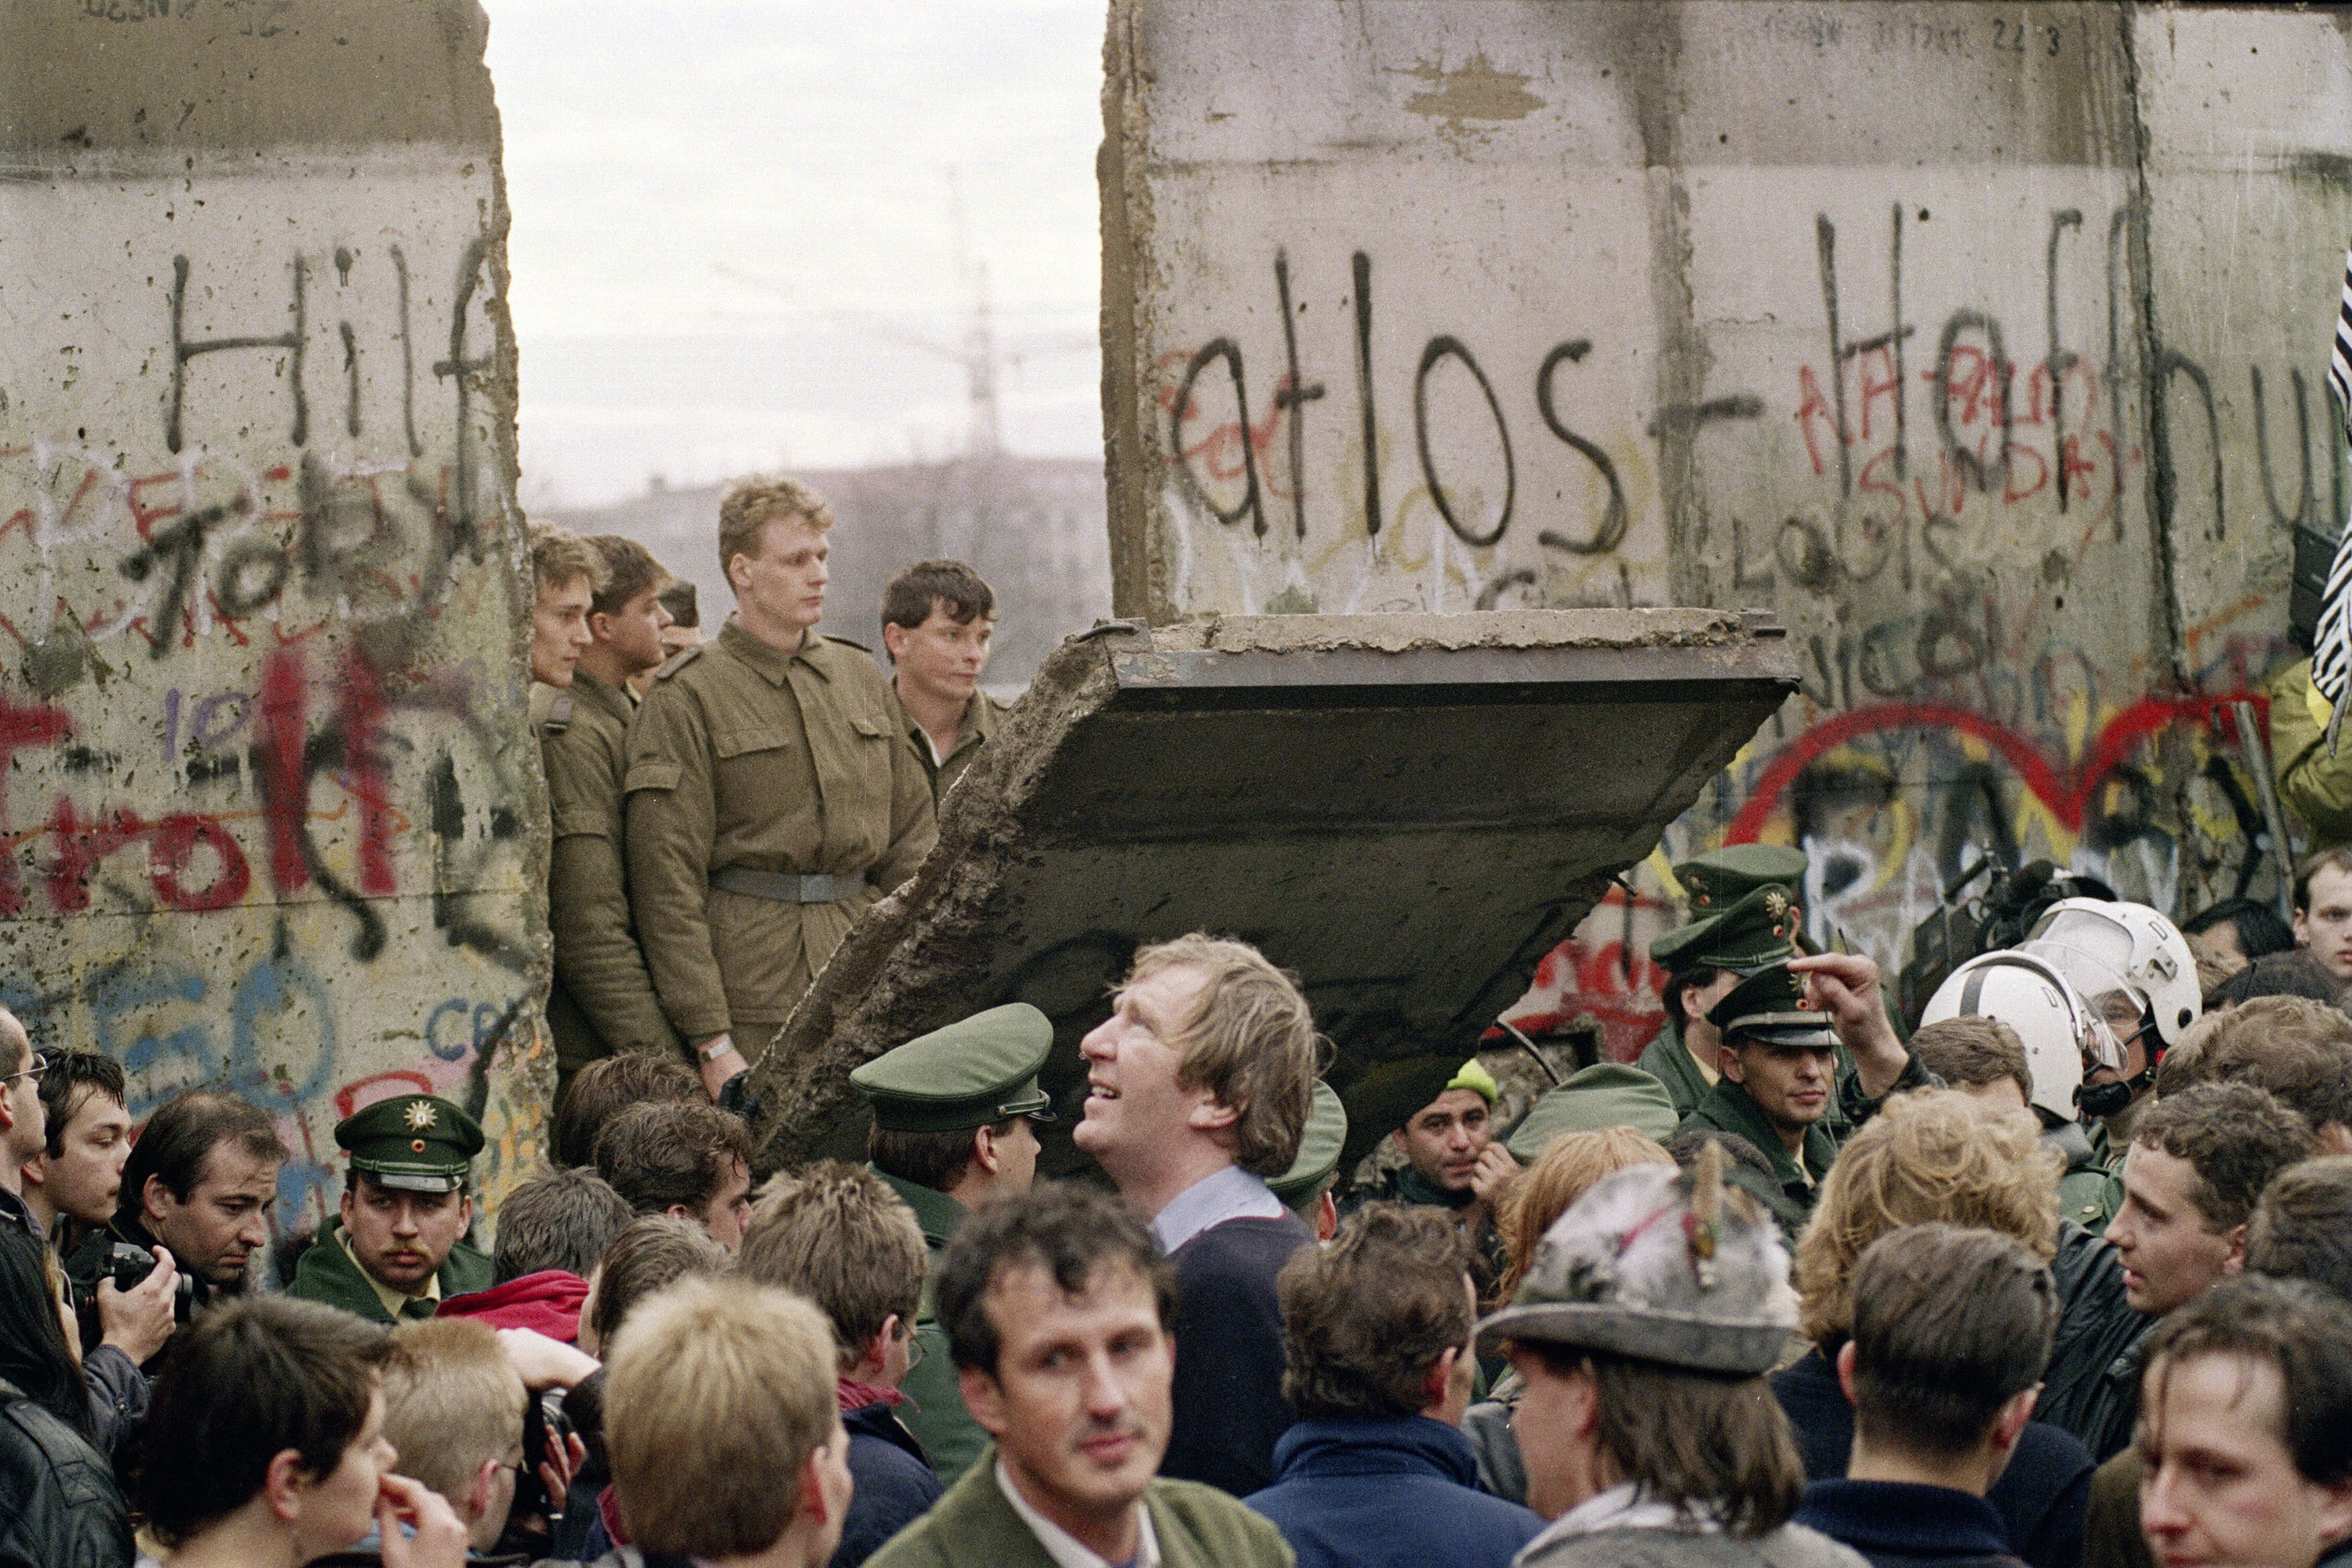
\includegraphics[keepaspectratio, height=\paperheight]{../img/berlin_wall_fall}};
  \end{tikzpicture}
\end{frame}
% ----------------------------------------------------
\note{Caída del Muro de Berlín, noviembre de 1989. Momento icónico del fin de la Guerra Fría.}

% ----------------------------------------------------
\begin{frame}
\frametitle{El fin de la Guerra Fría}
\centering

\begin{itemize}
  \item 1989: cae el Muro de Berlín
  \item 1991: se disuelve la Unión Soviética
  \item EE.UU. como única superpotencia
\end{itemize}

\end{frame}
% ----------------------------------------------------
\note{Gorbachev: glasnost y perestroika. 1989: revoluciones en Europa del Este. 1991: la URSS se disuelve en 15 Estados. Momento unipolar: EE.UU. sin rival. Optimismo: ``fin de la historia'' (Fukuyama). ¿Se cumplió?}

% ----------------------------------------------------
\begin{frame}[plain]
  \begin{tikzpicture}[remember picture, overlay]
    \node[at = (current page.center), yshift = 0cm] (cover) {%
      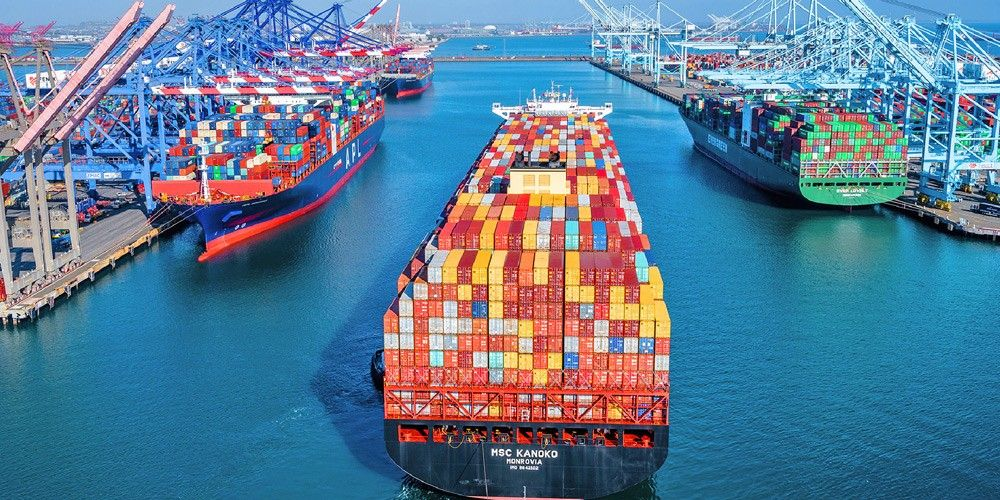
\includegraphics[keepaspectratio, height=\paperheight]{../img/container_ship}};
  \end{tikzpicture}
\end{frame}
% ----------------------------------------------------
\note{Barco de contenedores: símbolo de la globalización comercial. El comercio mundial se multiplica desde los 90.}

% % ----------------------------------------------------
% \begin{frame}
% \frametitle{La era de la globalización}
% \centering

% \begin{itemize}
%   \item Integración económica a escala global
%   \item Expansión de la UE, NAFTA, OMC
%   \item China y otros países se incorporan a la economía mundial
% \end{itemize}

% \end{frame}
% % ----------------------------------------------------

% ----------------------------------------------------
\begin{frame}[plain]
  \begin{tikzpicture}[remember picture, overlay]
    \node[at = (current page.center), yshift = 0cm] (cover) {%
      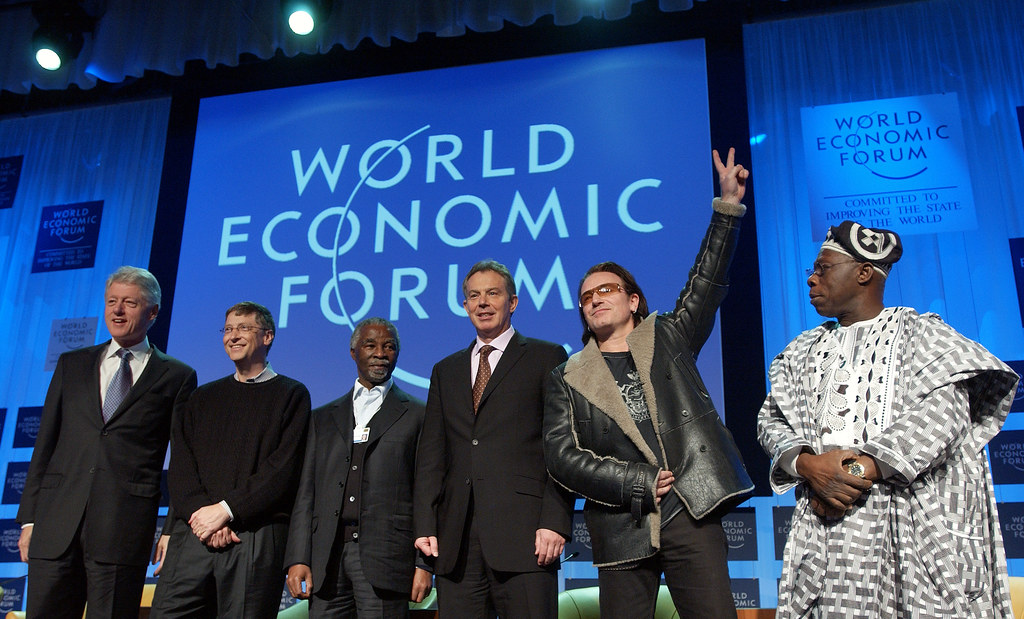
\includegraphics[keepaspectratio, height=\paperheight]{../img/davos2005}};
  \end{tikzpicture}
\end{frame}
% ----------------------------------------------------
\note{Foro Económico Mundial de Davos: símbolo de la gobernanza global y la globalización de élites. Expansión de la UE, creación del euro, NAFTA, OMC. China entra en la OMC en 2001.}

% ----------------------------------------------------
\begin{frame}[plain]
  \begin{tikzpicture}[remember picture, overlay]
    \node[at = (current page.center), yshift = 0cm] (cover) {%
      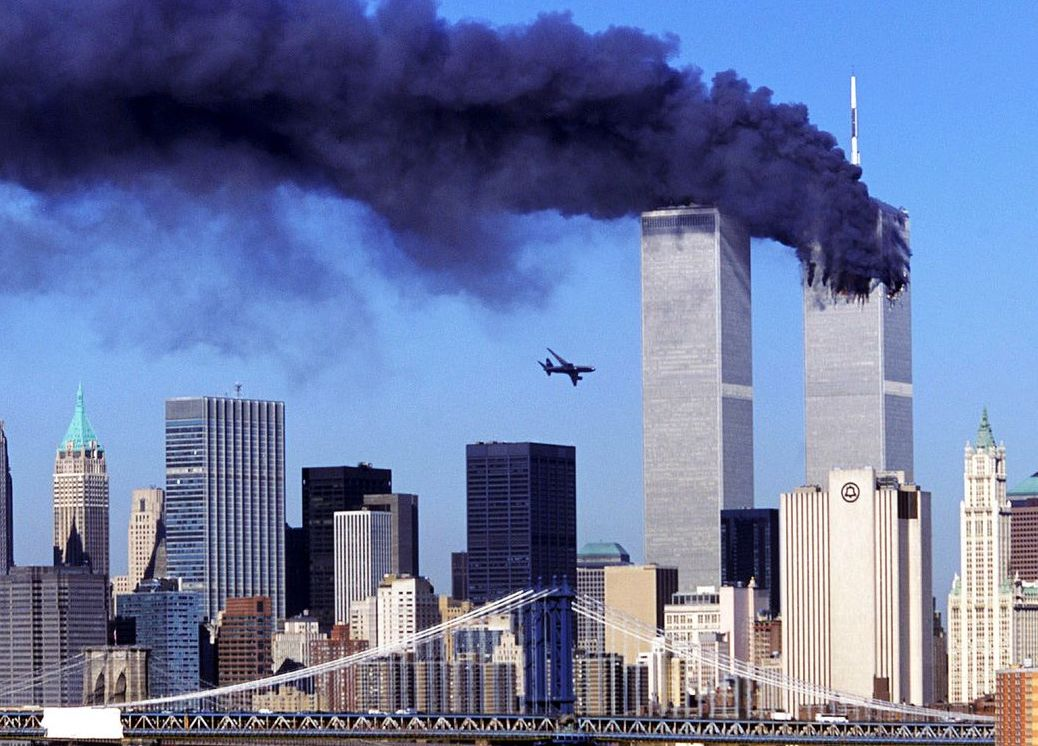
\includegraphics[keepaspectratio, height=\paperheight]{../img/september_11}};
  \end{tikzpicture}
\end{frame}
% ----------------------------------------------------
\note{11 de septiembre de 2001. Nuevo tipo de amenaza: terrorismo transnacional. Guerra de Afganistán (2001), Irak (2003). Década de intervenciones y ``guerra contra el terror''.}

% ----------------------------------------------------
\begin{frame}
\frametitle{Nuevos desafíos}
\centering

\begin{itemize}
  \item Terrorismo internacional (11-S, ISIS)
  \item Crisis financiera de 2008
  \item Populismo nacionalista y escepticismo ante la globalización
\end{itemize}

\end{frame}
% ----------------------------------------------------
\note{Crisis de 2008: la más grave desde los años 30. Austeridad, descontento social. Brexit (2016), Trump (2016): el populismo nacionalista cuestiona el orden liberal. ¿Fin del consenso pro-globalización?}

% ----------------------------------------------------
\begin{frame}[plain]
  \begin{tikzpicture}[remember picture, overlay]
    \node[at = (current page.center), yshift = 0cm] (cover) {%
      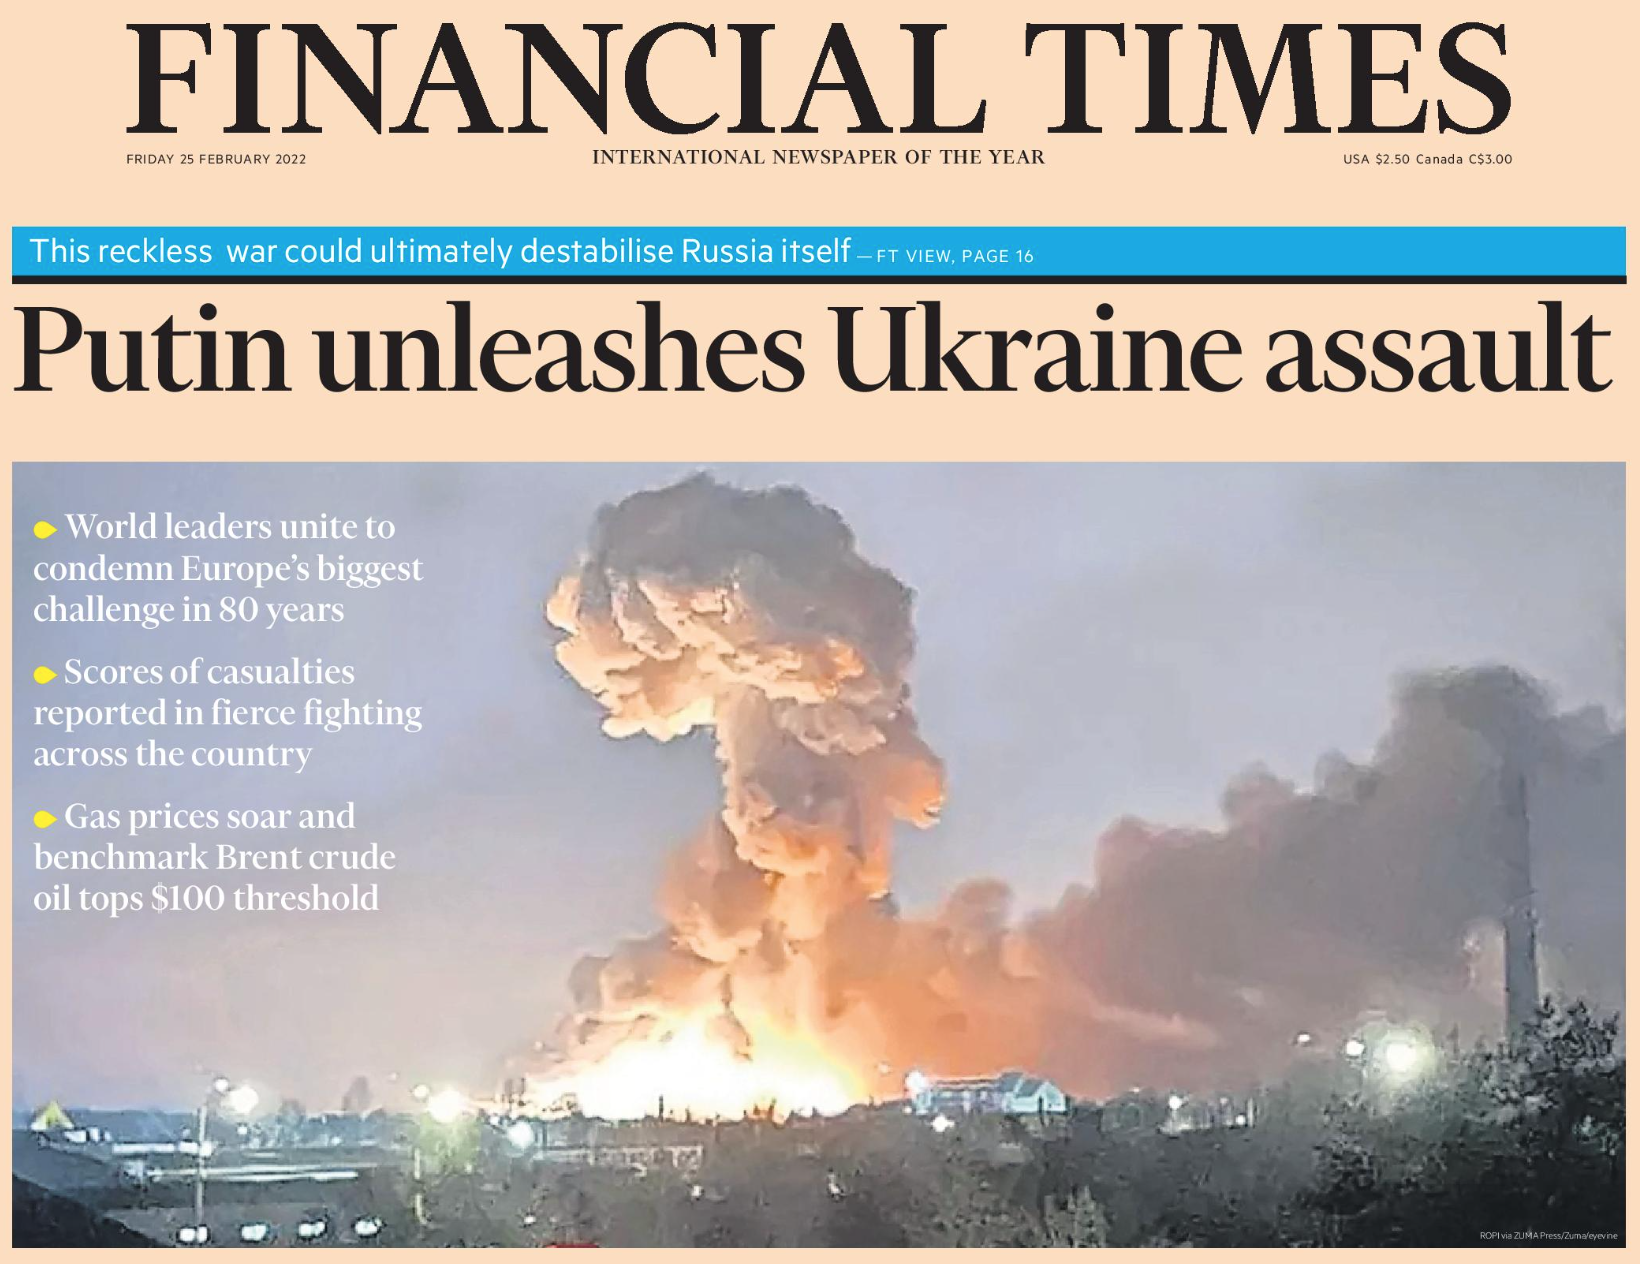
\includegraphics[keepaspectratio, height=\paperheight]{../img/ukraine_war}};
  \end{tikzpicture}
\end{frame}
% ----------------------------------------------------
\note{Guerra de Ucrania (desde 2022). Invasión rusa: el mayor conflicto en Europa desde 1945. Sanciones, reconfiguración geopolítica, crisis energética.}

% ----------------------------------------------------
\begin{frame}
\frametitle{El mundo hoy}
\centering

\begin{itemize}
  \item Guerras en Ucrania, Gaza, Sudán...
  \item Competición entre grandes potencias (EE.UU., China, Rusia)
  \item ¿Fin de la era de la globalización?
  \item ¿Estamos viviendo un momento más parecido a \textbf{1914} o a \textbf{1989}?
\end{itemize}

\end{frame}
% ----------------------------------------------------
\note{Pregunta final para discusión. ¿1914 (víspera de un conflicto catastrófico) o 1989 (transición hacia un nuevo orden)? No hay respuesta correcta: el objetivo es que piensen sobre los paralelismos históricos. Mencionar que el curso dará herramientas para analizar estas cuestiones.}

% ====================================================

% ----------------------------------------------------
\begin{frame}
\frametitle{}
\centering

Preguntas?

\end{frame}
% ----------------------------------------------------
\note{}
